\documentclass[aps,prd,longbibliography,reprint,twocolumn,amsmath,amssymb,amsfonts,showpacs,superscriptaddress]{revtex4-1}%reprint

\linespread{1.2}



\usepackage{graphicx, epsfig, amssymb}
\usepackage{amsmath, amsfonts}
\usepackage{bm}
\usepackage{enumitem}
\usepackage[usenames]{color}
\definecolor{navyblue}{rgb}{0.0, 0.0, 0.5}
\usepackage{hyperref}
\hypersetup
	{
		colorlinks,%
		citecolor=blue,%
		linkcolor=red,%
		urlcolor=blue,%
	}


%\usepackage[linktocpage,colorlinks=true,linkcolor=red]{hyperref}
\usepackage[caption=false]{subfig}
\usepackage[utf8]{inputenc}
\usepackage{tensor}
\usepackage{soul}
%\usepackage{enumerate}
\usepackage{pict2e}
\usepackage{diagbox}
\usepackage{empheq}

%\usepackage[margin=1in]{geometry}
\usepackage{float}
%\usepackage{subfig}
\usepackage{comment}
\usepackage{array}
%\usepackage{varioref}
%\usepackage[hidelinks]{hyperref}
%\usepackage{cleveref}
%\usepackage[numbers]{natbib}
\usepackage{units}
\usepackage{wasysym}
%\usepackage{caption}
%\usepackage{subcaption}



\DeclareMathAlphabet{\mathpzc}{OT1}{pzc}{m}{it}
\newcommand{\ff}{\hat{f}}

\def\l{\left}
\def\r{\right}
\def\p{\partial}

\newcommand{\angarg}{(\theta,\phi)}
\newcommand{\dth}{\frac{d}{d \theta}}
\newcommand{\sh}{ {}_{-s} S_{\ell m}^{a \omega}}
\newcommand{\zh}{ {}_{-s} Z_{\ell m}^{a \omega}}
\newcommand{\syjm}{  {}_{-s}Y_{jm} }
\newcommand{\sylm}{  {}_{-s} Y_{\ell m} }
\newcommand{\sumjm}{\sum_{j=s}^{\infty} \sum_{m=-j}^{j}}
\newcommand{\sumjms}{\sum_{j,m}}
\newcommand{\cS}{\mathcal{S}}
\newcommand{\lmws}{{\ell m \omega s}}
\newcommand{\nn}{\nonumber}

\newcommand*\widefbox[1]{\fbox{\rule[-2cm]{0pt}{4cm}\hspace{2em}#1\hspace{2em}}}

\newcommand{\sam}[1]{\textcolor{red}{(Sam: #1)}}
\newcommand{\tom}[1]{\textcolor{blue}{(Tom: #1)}}
\newcommand{\mo}[1]{\textcolor{green}{(Mohamed: #1)}}

\newcommand{\phiout}{\phi^{\text{out}}_{\omega, \lambda-1/2}}
\newcommand{\phireg}{\phi^{}_{\omega, \lambda-1/2}}

\renewcommand{\arraystretch}{1.3} % espace entre les lignes de la table
%\setlength{\tabcolsep}{.3cm} % espace entre les colonnes de la table

\usepackage{footnote}
\usepackage{tablefootnote}


\usepackage{threeparttable}


\begin{document}

\title{Scattering from compact objects: \\ Regge poles and the Complex Angular Momentum method}



\author{Mohamed \surname{Ould~El~Hadj}}
\email{m.ouldelhadj@sheffield.ac.uk}

\affiliation{Equipe Physique
Th\'eorique, SPE, UMR 6134 du CNRS
et de l'Universit\'e de Corse,\\
Universit\'e de Corse, Facult\'e des Sciences, BP 52, F-20250 Corte,
France}

\affiliation{Consortium for Fundamental Physics,  School of Mathematics and Statistics,
University of Sheffield, Hicks Building, Hounsfield Road, Sheffield S3 7RH, United Kingdom \looseness=-1}
%
\author{Tom Stratton}\email{tstratton1@sheffield.ac.uk}
\affiliation{Consortium for Fundamental Physics,  School of Mathematics and Statistics,
University of Sheffield, Hicks Building, Hounsfield Road, Sheffield S3 7RH, United Kingdom \looseness=-1}
%
\author{Sam R. Dolan}\email{s.dolan@sheffield.ac.uk}
\affiliation{Consortium for Fundamental Physics,  School of Mathematics and Statistics,
University of Sheffield, Hicks Building, Hounsfield Road, Sheffield S3 7RH, United Kingdom \looseness=-1}
%
\begin{abstract}
To be written
\end{abstract}

\date{\today}

\maketitle

\tableofcontents

\section{Introduction}

Change !

The time-independent scattering of planar waves in the gravitational field of a compact body has been studied in some detail since the 1960s \cite{Hildreth1964PhDT64, Matzner:1968, Vishveshwara:1970}. A substantial literature has developed on \emph{black hole scattering}, focussing on the canonical scenario of a planar wave of circular frequency $\omega$ and spin $s$ \cite{Chrzanowski:1976jb} impinging upon a black hole of mass $M$ in vacuum \cite{Hildreth1964PhDT64, Matzner:1968, Vishveshwara:1970, Mashhoon:1973zz,Fabbri:1975,Sanchez:1977vz,MatznerRyan1978,Handler:1980un,Matzner:1985rjn,Futterman:1988ni,Andersson:1995vi,Glampedakis:2001cx,Dolan:2006vj,Dolan:2007ut,Dolan:2008kf,Crispino:2009xt,Cotaescu:2014jca,Gussmann:2016mkp}. A dimensionless parameter
$
M \omega = \pi r_g / \lambda
$
encapsulates the ratio of the gravitational radius $r_g = 2GM/c^2$ to the wavelength $\lambda$ (we adopt geometric units such that $G=c=1$). The long wavelength ($M \omega \ll 1$), short wavelength ($M \omega \gg 1$) and intermediate regimes have been studied with a combination of perturbative \cite{DeLogi:1977dp,Dolan:2007ut,Guadagnini:2008ha,Sorge:2015yoa}, semi-classical \cite{Matzner:1985rjn, Anninos:1992ih} and numerical methods. The $s = 0$ (scalar) \cite{Matzner:1968,Sanchez:1977vz,Andersson:1995vi,Glampedakis:2001cx,Leite:2019eis}, $s=1/2$ (fermion) \cite{Dolan:2006vj,Cotaescu:2014jca}, $s=1$ (electromagnetic) \cite{Fabbri:1975, Crispino:2009xt, Crispino:2015gua} and $s=2$ (gravitational) cases \cite{MatznerRyan1978,Handler:1980un,Dolan:2008kf} have all been addressed.

Time-independent scattering by a compact body of radius $R$ with a regular centre, such as a neutron star or white dwarf, has received comparatively less attention. In such a scenario, an electromagnetic wave will not penetrate inside the compact body; but on the other hand, a gravitational wave will pass through the body without impediment from the matter distribution. Similarly, a neutron star is expected to be substantially transparent to neutrinos. However, even in these cases where the coupling to matter is negligible, the incident wave is still scattered by the influence of the spacetime curvature. Recent work \cite{Dolan:2017rtj, Stratton:2019deq} explored the \emph{rainbow scattering} phenomenon that arises at short wavelengths, due to a stationary point in the geodesic deflection function associated with a ray that passes somewhat inside the body. In principle, the rainbow angle is a diagnostic of the matter distribution of the body, and thus its nuclear equation of state. Indeed, in the 1970s, experimental data on rainbows in nucleon-nucleon scattering experiments was used to constrain models of the nuclear potential.

Other recent works have examined scattering from a compact object with an absorbing surface \cite{Nambu:2019sqn}; and scattering simulations using finite-element-method codes \cite{He:2019orl}.

The tenuity (inverse compactness) .

Now describe the application of CAM methods to black holes, and its successes ... The aim of this work is to extend the methods to compact bodies.

Describe QNMs - resonances in the time domain: \cite{Detweiler:1985zz, Kokkotas:1986gd, Chandrasekhar449, Kokkotas:1992ka, Leins:1993zz, Andersson:1995ez, Andersson1996} Review of QNMs: \cite{Kokkotas:1999bd}. Now describe how these are connected to Regge poles.

Finally a paragraph on the connections to Mie scattering by a transparent sphere.

\cite{Leite:2017zyb,Nambu:2019sqn, Folacci:2019vtt,}.





%\section{Differential scattering cross sections for scalar waves, their CAM representation and their Regge pole approximations}
\section{Waves on a compact-body spacetime}
\label{SecII}


In this section we describe the model for the compact object (\ref{SecIIa}); we introduce the effective potentials for scalar field and axial gravitational waves (\ref{subsec:Potentials}); and we define the physical boundary conditions and the S-matrix (\ref{subsec:bc}).

%Finally we apply the CAM-approach developed for black-hole scattering in \cite{Folacci:2019cmc} and \cite{Folacci:2019vtt}.

\subsection{The model}
\label{SecIIa}

The gravitating source is assumed to be spherically-symmetric, such that in a coordinate system $\{t,r,\theta,\varphi\}$, the object is described by a diagonal metric $g_{\mu \nu}$ and the line element
\begin{equation}\label{Line_elem}
 ds^2 = g_{\mu \nu} dx^\mu dx^\nu = -f(r) dt^2+h(r)^{-1}dr^2+r^2d\sigma_2^2
\end{equation}
where $d\sigma_2^2 = d\theta^2 + \sin^2 \theta d\varphi^2$ denotes the metric on the unit 2-sphere $S^2$. In the vacuum exterior of the star ($r>R$), the radial functions $f(r)$ and $h(r)$ depend only on $M$, the total mass of body: $f(r)=h(r)=1-2M/r$ by Birkhoff's theorem~\cite{VojeJohansen:2005nd}. In the interior, $f(r)$ and $h(r)$ depend on the matter distribution and equation of state (EoS).

A widely-studied model is that of a polytropic star, with an EoS $p(\rho) = \kappa \rho^{1+1/\hat{n}}$, where $\hat{n}$ is the polytropic index (see e.g.~\cite{Stratton:2019deq}). Here we shall consider a special case: an incompressible perfect fluid ball of uniform density described by Schwarzschild's interior solution for an incompressible fluid \cite{Shapiro1983}, with
\begin{subequations}
\begin{align}
\rho &= \frac{M}{\frac{4}{3} \pi R^3} , \\
p &= \rho \frac{\beta(R) - \beta(r)}{ \beta(r) - 3 \beta(R)} , \\
\beta(x) &= \sqrt{3 - 8 \pi \rho x^2}
\end{align}
\end{subequations}
and metric functions
%
\begin{subequations}\label{Interior_Solution}
\begin{align}\label{Interior_Solution_f}
 f(r) &= \frac{1}{4}\left(1-\frac{2 M r^2}{R^3}\right)+\frac{9}{4}\left(1-\frac{2M}{R}\right) \nn \\
       & \quad -\frac{3}{2} \sqrt{\left(1-\frac{2M}{R}\right)\left(1-\frac{2 M r^2}{R^3}\right)}, \\
 h(r) &= 1-\frac{2 M r^2}{R^3} . \label{Interior_Solution_h}
\end{align}
\end{subequations}
The constant-density model can be thought of as representing the $\hat{n} \rightarrow 0$ limit of the family of polytropes.
The radial function $h(r)$ is $C^0$ at the surface of the star $r=R$ (i.e.~continuous but not differentiable), and the radial function $f(r)$ is $C^1$ there (i.e.~once-differentiable). In the polytropic cases $n > 0$, the functions are more regular \sam{can we make a precise statement?} at the surface, but not $C^\infty$ (i.e.~not smooth). As we shall see, the breakdown of smoothness leads to consequences for the Regge pole spectrum.

We shall consider a scalar wave $\Phi(x)$ propagating on the compact body spacetime, governed by the Klein-Gordon equation
\begin{equation}
\Box \Phi \equiv \frac{1}{\sqrt{-g}} \partial_{\mu} \left( \sqrt{-g} g^{\mu \nu} \partial_{\nu} \Phi \right) = 0
\end{equation}
where $g^{\mu \nu}$ is the inverse metric and
$
g % = - f(r) h^{-1}(r) r^4 \sin^2 \theta
$
 is the metric determinant. Performing a standard separation of variables,
\begin{equation}
\Phi = \frac{1}{r} \sum_{\omega \ell m} \phi_{\omega \ell}(r)  Y_{lm}(\theta, \phi) e^{-i \omega t} ,
\label{eq:sepvariables}
\end{equation}
leads to a radial equation of the form
\begin{equation}
\label{H_Radial_equation}
\left[\frac{d^{2}}{dr_{\ast}^{2}}+\omega^{2}-V_{\ell}(r)\right]\phi_{\omega\ell}= 0,
\end{equation}
where $V_{\ell}(r)$ is the effective potential, and $r_\ast$ denotes the \emph{tortoise coordinate} defined by
\begin{equation}
\frac{dr}{dr_\ast} =\sqrt{f(r)h(r)} .  \label{eq:tortoise}
\end{equation}

\subsection{Effective potentials}\label{subsec:Potentials}
The effective potential for the scalar field in Eq.~(\ref{H_Radial_equation}) is $V_{\ell}(r) = V_{\ell}^{(s=0)}(r)$, where we define
\begin{equation}\label{Inside_Potentiel}
  V_{\ell}^{(s)}(r) \equiv f(r)\left[\frac{\ell(\ell+1)}{r^2}+\frac{\beta_s \, h(r)}{2r}\left(\frac{f'(r)}{f(r)}+\frac{h'(r)}{h(r)}\right)\right] ,
\end{equation}
where $\beta_s \equiv 1-s^2$.
Remarkably, the radial equation for axial gravitational perturbations is identical to Eq.~(\ref{H_Radial_equation}) but with an effective potential $V_{\ell}^{\text{ax}}(r)$ where \cite{Cardoso:2014sna}
\begin{eqnarray}\label{RW_Potentiel_axialGW}
V_{\ell}^{\text{ax}}(r) = V_{\ell}^{(s=2)} + 8 \pi f(r) (p - \rho)  .
\end{eqnarray}
%
Outside the star in the vacuum region ($r>R$), the effective potentials reduce to the Regge-Wheeler potential,
\begin{equation}\label{RW_Potentiel}
V^{(s)}_{\ell}(r) =\left(1-\frac{2M}{r}\right)\left(\frac{\ell(\ell+1)}{r^2}+\frac{2M \beta_s}{r^3}\right)
\end{equation}
with $s=0$ in the scalar-field case, and $s=2$ in the axial gravitational-wave case. In the exterior, the tortoise coordinates $r_\ast$ reduces to $r_\ast = r+ 2M \ln [r/(2M) -1]+k$, where $k$ is a constant that is chosen such that $r_\ast(r=0) = 0$ and $r_\ast(r)$ is a continuous function.

Effective potentials for the incompressible model are shown in Fig.~\ref{fig:Veff}, for two cases: (i) a neutron-star model with $R = 6M$, and (ii) a ultra-compact object (UCO \cite{Macedo:2018yoi}) with $R = 2.26M$. % (i.e.~close to the Buchdahl bound of $R/M = 9/4$).
In both cases we observe a discontinuity in $V_{\ell}(r)$ across the star's surface, due to the $C^0$ property of $h(r)$. The jump in the potential takes opposite signs in the scalar-field and gravitational-wave cases, with
\begin{subequations}
\begin{align}
\Delta V_{\ell}^{(s=0)} &= + \frac{3Mf(R)}{R^3} , \\
\Delta V_{\ell}^{\text{ax}} &= - \frac{3Mf(R)}{R^3} ,
\end{align}
\end{subequations}
where
\begin{equation}
\Delta V_{\ell} \equiv \lim_{\epsilon \rightarrow 0} \left\{ V_{\ell}(R + \epsilon) - V_{\ell}(R - \epsilon) \right\} . \label{def:DeltaV}
\end{equation}


 \begin{figure}[htb]
\centering
 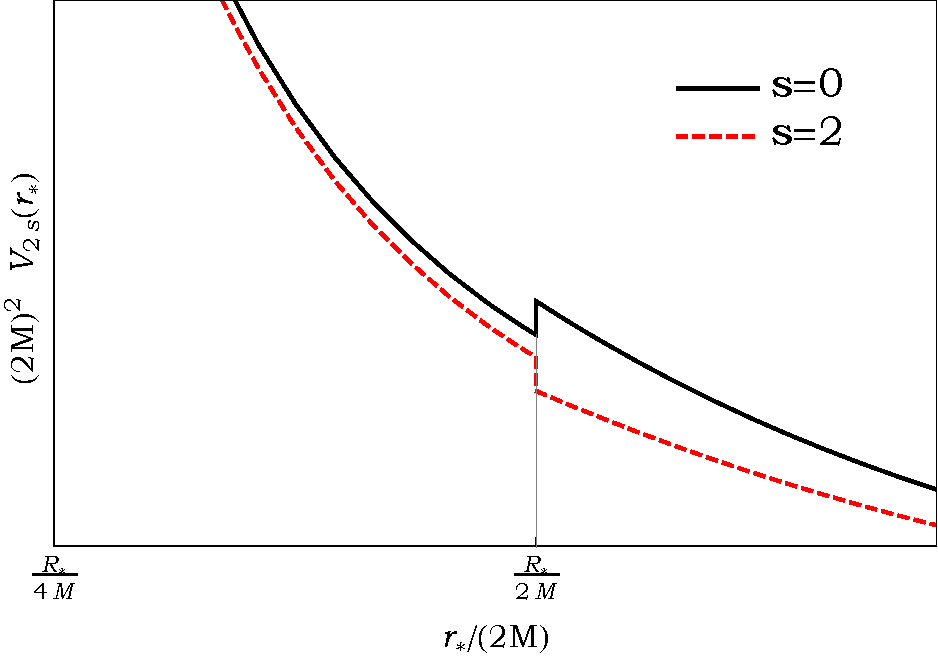
\includegraphics[scale=0.50]{potentials_s02_CD_R6L2_v3} \\ \vspace{0.2cm}
 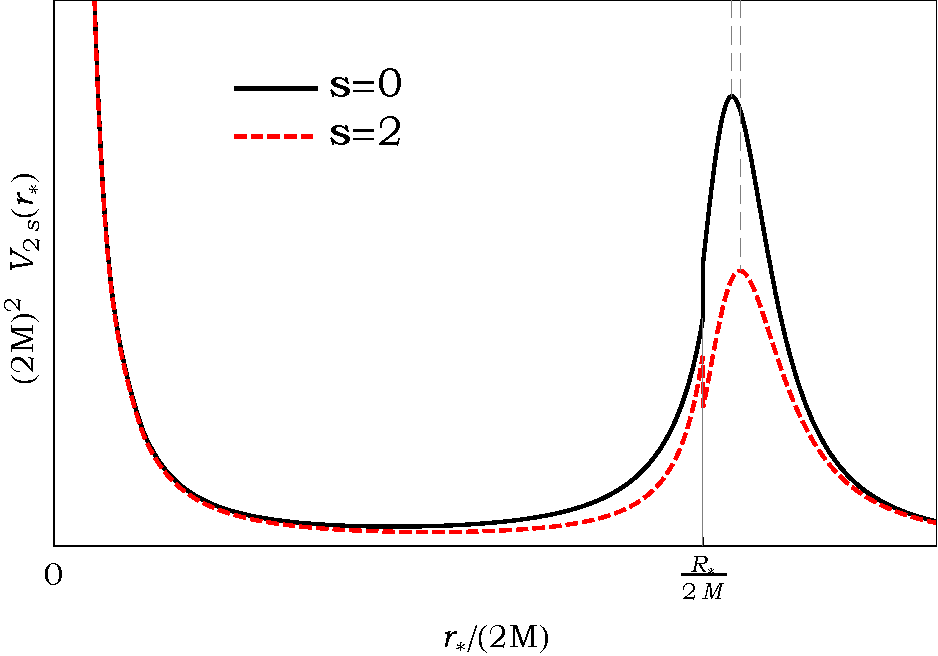
\includegraphics[scale=0.50]{potentials_s02_CD_R2p26L2_v3}
\caption{\label{RP_approx_2Mw_3_6_s_1} The effective potential $V_\ell$ for a quadrupole ($\ell =2$) perturbation of a compact body of constant density and tenuity $R/M = 6$ (upper) and $R /M = 2.26$ (lower). The scalar field potential (\ref{Inside_Potentiel}) and axial gravitational-wave potential (\ref{RW_Potentiel_axialGW}) are indicated as solid/black lines and dotted/red lines, respectively. The horizontal axis is the tortoise coordinate $r_\ast/(2M)$ defined in Eq.~(\ref{eq:tortoise}).}
\label{fig:Veff}
\end{figure}

In the UCO case ($R < 3M$), the effective potential has a maximum near the light-ring at $r=3M$, and there is a trapping region, as shown in Fig.~\ref{fig:Veff}.

\subsection{Boundary conditions and scattering}\label{subsec:bc}
The modes $\phi_{\omega \ell}$ in Eq.~(\ref{eq:sepvariables}) should have a regular behaviour at the centre of the object ($r = 0$), and inspection of the radial equation (\ref{H_Radial_equation}) shows that
\begin{equation}\label{bc_1_in}
\phi_{\omega  \ell}(r) \, \scriptstyle{\underset{r \to 0}{\sim}} \,
\displaystyle{r^{\ell+1}}.
\end{equation}
At the boundary of the compact object, the potential is $C^0$ and thus the mode is $C^2$.
The asymptotic behaviour of the modes far from the body ($r \to +\infty$, or equivalently $r_\ast \to +\infty$) is
\begin{equation}\label{bc_2_in}
\phi_{\omega  \ell}(r) \scriptstyle{\underset{r_\ast \to +\infty}{\sim}}
\displaystyle{ A^{(-)}_\ell (\omega) e^{-i\omega r_\ast} + A^{(+)}_\ell (\omega) e^{+i\omega r_\ast}}.
\end{equation}
With the complex coefficients $A^{(\pm)}_\ell (\omega)$ we then define the \emph{S-matrix elements},
\begin{equation}\label{Matrix_S}
  S_{\ell}(\omega) =  e^{i(\ell+1)\pi} \, \frac{A_{\ell}^{(+)}(\omega)}{A_{\ell}^{(-)}(\omega)}.
\end{equation}
We now consider the poles of $S_{\ell}(\omega)$ in the complex plane.

%We can expect then that Regge poles for axial gravitational perturbations are qualitatively the same as for scalar perturbations, and the methods discussed can be easily adapted to deal with either case.

\section{The Regge pole spectrum}

 \subsection{Quasinormal modes and Regge poles}
 Mathematically, there is a close relationship between quasinormal modes and Regge poles; they are both sets of poles of the scattering matrix. Physically, quasinormal modes are most relevant to time-dependent scattering scenarios, and Regge poles to time-independent scattering scenarios.

The \emph{quasinormal mode spectrum} is the set of frequencies $\{ \omega_{\ell n} \}$ in the complex-$\omega$ plane at which the scattering matrix $ S_{\ell}(\omega)$ has a simple pole for a integer value of $\ell$ (so $\ell \in \mathbb{N}$ and $\omega_{\ell n} \in \mathbb{C}$).

The \emph{Regge pole spectrum} is the set of angular momenta $\lambda_{n}(\omega) = \ell_{n}(\omega) + 1/2$ in the complex-$\lambda$ plane at which the scattering matrix has a simple pole for a real value of $\omega$ (so $\omega \in \mathbb{R}$ and $\lambda_{n}(\omega) \in \mathbb{C}$). Here $n$ is an index for enumerating the discrete spectrum of poles. In all cases considered in this work, the simple poles of $S_{\ell}(\omega)$ arise as simple zeros of $A_{\ell}^{(-)}(\omega)$.

The quasinormal mode spectrum of spherically-symmetric compact objects has been studied in some detail in Refs.~\cite{Kokkotas:1986gd,Kokkotas:1992ka,Andersson:1997eq,Kokkotas:1999bd,Leins:1993zz}.
Newly-formed neutron stars, the remnants of supernovae collapse, are predicted to pulsate with a large initial energy, and fluid pulsations will generate gravitational waves. In 1967, Thorne and Campolattaro \cite{thorne1967non} classified the fluid modes of a relativistic compact body by analogy with the fluid modes of a Newtonian body, with the addition of a damping time due to the emission of GWs. Two decades later, the subject was examined again \cite{Detweiler:1985zz,Kokkotas:1986gd}, and Kokkotas and Schutz \cite{Kokkotas:1992ka} showed the existence of an additional family of modes, dubbed $w$-modes. These modes are characterised by a negligible excitation of fluid motion, and in the axial sector, by no fluid motion at all. They are highly damped and correspond to excitations of the dynamical perturbed space-time. For a review of (gravitational) quasinormal modes in relativistic stars and black holes see Ref.~\cite{Kokkotas:1999bd}.

The $w$-modes (quasinormal modes) may be divided into three branches:
	\begin{enumerate}
   \item Curvature modes, oscillations whose damping is larger for less compact bodies. \sam{Anything else to say on curvature modes?}
   \item Interface modes ($\omega_{\text{II}}$-modes \cite{Leins:1993zz}), characterised by very rapid damping (i.e.~large negative imaginary part of $\omega_{\ell n}$). This branch of modes is most similar to the Schwarzschild black hole quasinormal modes.
   \item Trapped modes \cite{Chandrasekhar449}: These modes exist for UCOs with $R/M < 3$, because the effective radial potential has a local minimum inside the star, and local maximum near the photon sphere $r=3M$. %The trapped modes are essentially the first few curvature modes with energy less than the potential barrier.
   The number of trapped modes increases with the depth of the potential well, and the damping rate decreases.
	\end{enumerate}
For more details on quasinormal modes see \sam{Appropriate reference needed.}

We now turn our attention to calculating the Regge pole spectrum for compact bodies.


 \subsection{Numerical method}\label{subsec:method}


In order to determine the Regge poles we adapt the method of Benhar, Berti and Ferrari (BBF), described in Sec.~4 of Ref.~\cite{Benhar:1998au}. In turn, the BBF method is an adaptation of the \textit{continued fraction method} developed by Leaver in the case of black hole-quasinormal mode frequencies~\cite{Leaver:1985ax}. Though BBF used the method to find axial QNM frequencies, their method is equally valid, \textit{mutatis mutandis}, for finding the Regge poles $\{\lambda_n(\omega)= \ell_n +1/2\}$ of $ S_{\ell}(\omega)$. BBF write the solution of the Regge-Wheeler equation in a power-series form as follows:
%\begin{equation}\label{Power_series}
%  \phi_{\omega_\ell}(r) =\left(\frac{r}{2M}-2M\right)^{i 2M\omega} \,e^{i\omega r} \sum_{n,=0}^{+\infty}a_n\left(1-\frac{b}{r}\right)^n
%\end{equation}

\begin{eqnarray}\label{Power_series}
% \nonumber % Remove numbering (before each equation)
 \phi_{\omega_\ell}(r)&=&\left(\frac{r}{2M}-2M\right)^{i 2M\omega} \,e^{i\omega r} \sum_{n,=0}^{+\infty}a_n\left(1-\frac{b}{r}\right)^n \nonumber \\
                      &=& e^{i\omega r_*(r)}\sum_{n,=0}^{+\infty}a_n\left(1-\frac{b}{r}\right)^n
\end{eqnarray}
where $r = b$ is some point outside the star. By substituting \eqref{Power_series} in the Regge-Wheeler equation, BBF found that the coefficients $a_n$ satisfy a four–term recurrence
relation of the form:
\begin{equation}\label{Recurrence_4_terms}
\alpha_n a_{n+1} + \beta_n a_{n} +\gamma_{n} a_{n-1} +\delta_{n} a_{n-2}  = 0, \quad \forall n\geq 2
\end{equation}
where
\begin{eqnarray}\label{Coeffs_3_termes}
 && \alpha_n = n (n+1)\left(1-\frac{2M}{b}\right)   \\
 && \beta_n  = 2i\omega b n + 3\left(\frac{2M}{b}\right)n^2-2n^2  \\
 && \gamma_n = \left(1-\frac{6M}{b}\right)n(n-1)-\beta_s\left(\frac{2M}{b}\right)-\ell(\ell+1)  \\
 && \delta_n = \left(\frac{2M}{b}\right)\left(n(n-2)+\beta_s\right)
\end{eqnarray}
To determine the initial conditions $a_0$ and $a_1$, we impose the continuity of $\phi_{\omega_\ell}(r)$ and its derivative in $r = b$, according to Eq~\eqref{Power_series}, we obtain:
\begin{eqnarray}\label{Initial_Conds}
 && a_0 = e^{i\omega r_*(b)\phi_{\omega_\ell}(b)}  \\
 && a_1 = b e^{-i\omega r_*(b)}\left(\frac{-i\omega b}{b-2M}\phi_{\omega_\ell}(b)+ \frac{d}{dr}\phi_{\omega_\ell}(r)\Big{|}_{r=b}\right)
\end{eqnarray}
Here, to obtain $\phi_{\omega_\ell}(b)$ and its derivative in $r=b$, we need to solve numerically the Eq.~\eqref{H_Radial_equation} inside the star and to continue the solution outside, up to $r=b$, by solving the Regge-wheeler equation.

It is important to note that, the \textit{continued fraction method} is applied to the three-term recurrence relation. To do this, BBF has used the method introduced by Leaver in
the case of Reissner-Nordstöm   black hole \cite{Leaver:1990zz}, \textit{i.e.}, reducing the four-term recurrence relations \eqref{Recurrence_4_terms} to a three-term recurrence relation by using the gaussian elimination step.

We have implemented numerically this method by using the \textit{Hill determinant approach} of Majumdar and Panchapakesan~\cite{mp} introduced in the case of Schwarzschild black hole. They gave an alternative condition and they suggested that the nontrivial solutions of \eqref{Recurrence_4_terms} exists  when the Hill determinant vanish:
\begin{equation}
\label{Determinant_Hill_4_termes}
D   =  \begin{vmatrix}
   \beta_0         &  \alpha_0    &        0             &       0                    &          0                &     \ldots          &     \ldots        &    \ldots \\
   \gamma_1        &  \beta_1      &     \alpha_1     &       0                    &          0                &     \ldots          &     \ldots        &    \ldots  \\
    \delta_2       &   \gamma_2     &    \beta_2       &   \alpha_2             &         0                &     \ldots           &    \ldots         &    \ldots  \\
    \vdots         &      \ddots     &     \ddots       &    \ddots                &       \ddots          &     \ddots           &   \ldots          &    \ldots \\
     \vdots        &     \vdots      &     \delta_{n-1}      &    \gamma_{n-1}      &     \beta_{n-1}     &      \alpha_{n-1} &    \ddots         &    \ldots  \\
     \vdots        &  \vdots        &     \vdots        &     \delta_n                &    \gamma_{n}    &     \beta_{n}        &     \alpha_{n}  &    \ddots     \\
     \vdots        &  \vdots        &     \vdots        &     \vdots                &    \ddots            &     \ddots            &     \ddots       &    \ddots
                        \end{vmatrix}
       = 0
\end{equation}



 \subsection{Numerical results: the spectrum}\label{subsec:results1}
In this section we show numerical results for the Regge pole spectrum of a compact body, in two particular cases: (i) a neutron-star-like body with tenuity $R / M = 6$, and (ii) a UCO with tenuity $R / M = 2.26$ close to the Buchdahl bound. Results for the frequencies $M \omega = 3/2$ and $M \omega = 8$ are compared, for the scalar-field ($s=0$) and axial GW ($s=2$) cases.

Figure \ref{fig:rp1} shows the Regge pole spectrum for a neutron-star-like body ($R/M = 6$). We see that there are two branches of Regge poles in the first quadrant, which meet at $\text{Re}( \lambda_n(\omega) ) \sim \omega b_0$, where $b_0$ is the impact parameter for the null ray which grazes the surface of the compact body. The axial GW $s=2$ modes (filled markers) are typically close to their scalar-field $s=0$ counterparts (unfilled markers), as might be anticipated from the similarities in the effective potentials for the two cases (see Fig.~\ref{fig:Veff}).

\begin{figure}[htb]
\centering
 \includegraphics[scale=0.50]{RP_R_6_2Mw_3_16_s_0_s_2}
\caption{\label{RP_approx_2Mw_3_6_s_1} The Regge poles $\lambda_n(\omega)$ for the scalar field (empty markers) and for the axial gravitational waves (filled markers). %We assume $2M =1$.
}
\label{fig:rp1}
\end{figure}

Figure \ref{fig:rp2} shows the spectrum for a UCO with $R/M = 2.26$. These plots show evidence for an additional branch of modes that emerges from the point where the first two branches meet. The number of modes in this branch increases as the radius of the body approaches the Buchdahl limit $R \rightarrow \tfrac{9}{4}M$.

 \begin{figure}[htb]
\centering
 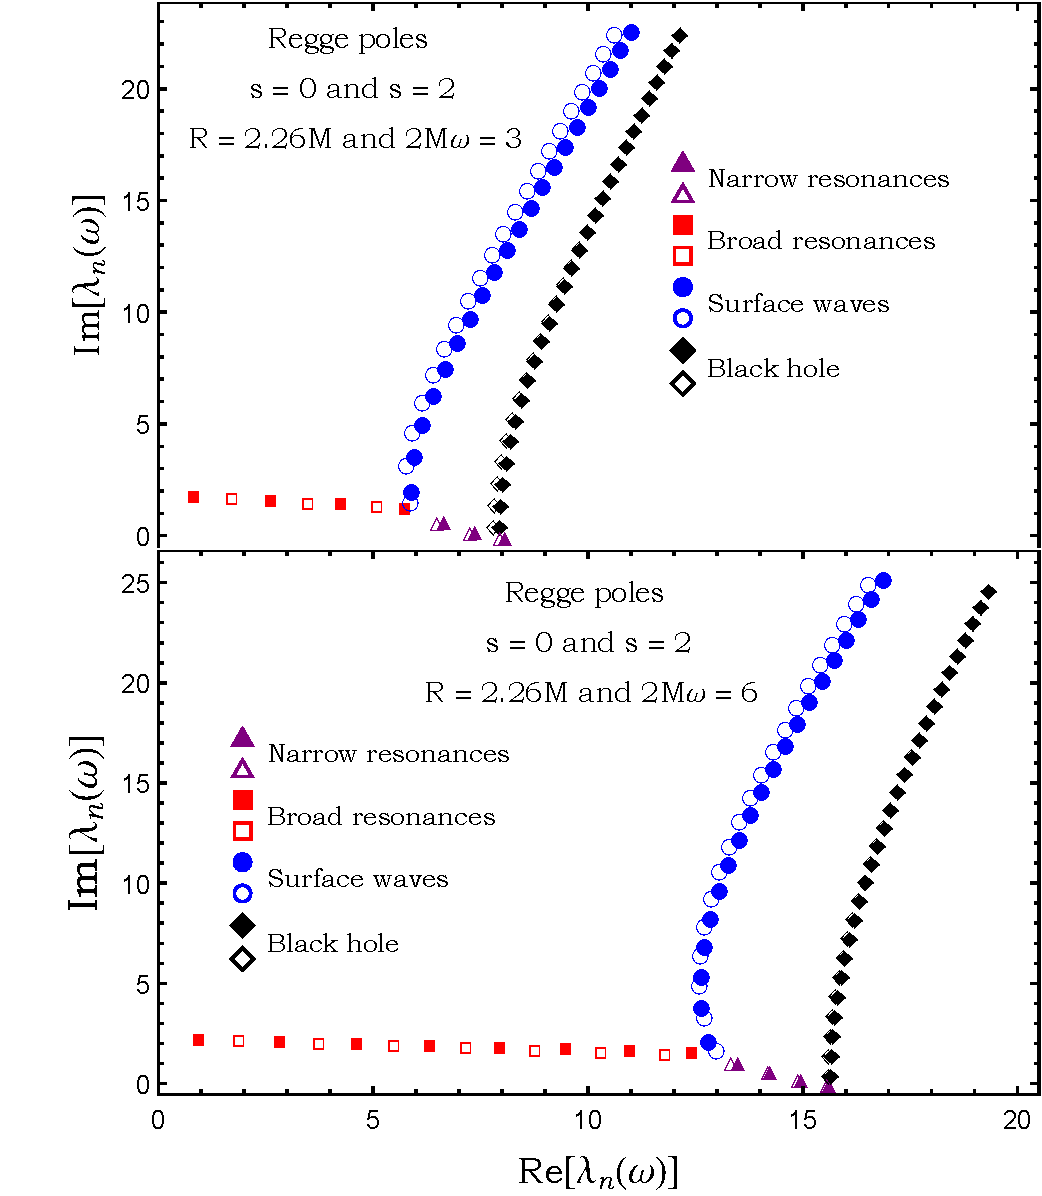
\includegraphics[scale=0.50]{RP_R_2_dot_26_2Mw_3_6_s_0_s_2}
\caption{\label{RP_approx_2Mw_3_6_s_1}  The Regge poles $\lambda_n(\omega)$ for the scalar field (empty markers) and for the axial gravitational waves (filled markers). %We assume $2M =1$.
}
\label{fig:rp2}
\end{figure}

The Regge pole spectrum for a compact body is qualitatively similar to the Regge pole spectrum found in Mie scattering of electromagnetic waves by a transparent droplet of refractive index $\tilde{n}$. This has been studied since the 1960s; see for example Fig.~9.2 in Ref.~\cite{Nussenzveig:2006}. % In the latter case, the poles are given by the zeros of a combination of special functions.
Henceforth we shall adopt the terminology of Nussenzveig \cite{Nussenzveig:2006}, in which the three branches are labelled as:
\begin{enumerate}
 \item \emph{Broad resonances}: approximately uniformly-spaced poles above the real axis with approximately constant imaginary part; somewhat sensitive to internal structure ($r < R$);
 \item \emph{Surface waves}: highly-damped modes that are relatively insensitive to the internal structure and which depend chiefly on the surface geometry.
 \item \emph{Narrow resonances}: modes approaching the real axis corresponding to trapped modes which only appear in the UCO case ($R < 3M$).
\end{enumerate}
In Figs.~\ref{fig:rp1} and \ref{fig:rp2} the broad resonances, surface waves and narrow resonances are indicated by red squares, blue circles and purple triangles, respectively; and black diamonds indicate the black hole RPs. Whereas there exists an infinite number of poles of the surface-wave branch, in principle, there are no narrow-resonance poles at all in the $R/M = 6$ case, and just $\le 4$ narrow-resonance poles in the $R/M = 2.26$ case. The narrow-resonance branch is observed to end close to the start of the black-hole branch.

Data for Regge poles $\lambda_n(\omega)$ is listed in Table \ref{tab:table1} (scalar field, $R/M=6$), Table \ref{tab:table2} (scalar field, $R/M = 2.26$), Table \ref{tab:table3} (axial $s=2$, $R/M = 6$) and Table \ref{tab:table4} (axial $s=2$, $R/M = 2.26$). The values are labelled by branch (broad; surface; narrow). For the scalar field, the associated residues (see Sec.~) are also presented in Tables \ref{tab:table1} and Table \ref{tab:table2}.

\begingroup
\squeezetable
\begin{table*}[htp]
\begin{threeparttable}[htp]
%\captionsetup{font=small}
\caption{\label{tab:table1} The lowest Regge poles $\lambda_{n}(\omega)$ for the scalar field and the associated residues $r_{n}(\omega)$. The radius of the compact bodies is $R = 6M$.}
\smallskip
\centering
\begin{ruledtabular}
\begin{tabular}{cccccc}
 $n$ & $2 M \omega$  & $\lambda^{\text{(S-W)\tnote{1}}}_n(\omega)$ & $\lambda^{\text{(B-R)\tnote{2}}}_n(\omega)$ & $r^{\text{(S-W)}}_{n}(\omega)$ & $r^{\text{(B-R)}}_{n}(\omega)$
 \\ \hline
$1$  & $3$  & $ 9.64850+2.76784 i$  & $1.56219+2.33072 i$  & $-12.41483-0.10424 i$  & $ -0.184457+0.480330 i$    \\
     & $16$  & $56.00945+5.71038 i$  & $ 0.62529+3.27098 i$  & $-447.5395+25.2912 i$  & $-0.322061-0.088002 i $  \\

$2$  & $3$  & $ 10.71986+5.16209 i $  & $3.81484+2.48159 i$  & $13.8486+24.3824 i$  & $0.290952+1.043116 i$    \\
     & $16$  & $ 58.442656+9.18793 i$ & $2.64868+3.31439 i$  & $5188.750-859.909 i$  & $ -0.381581-0.077583 i$    \\

$3$  & $3$  & $11.62296+7.17454 i$  & $ 6.35675+2.64104 i$  & $39.4189-12.3554 i$ & $2.83038-0.28686 i$    \\
     & $16$  & $60.20374+12.14965 i$  & $4.70011+3.35821 i$  & $-29331.71-18578.38 i$  & $-0.456423-0.021249 i$ \\

$4$  & $3$  & $ 12.4297+8.9960 i$  & $/$  & $ 13.2301-50.8802 i$ & $/$    \\
     & $16$  & $ 61.67700+14.84728 i $  & $6.78093+3.40257 i$  & $-15868.9+161199.9 i$  & $-0.528929+0.106794 i$ \\

$5$  & $3$  & $13.1734+10.6929 i$  & $/$  & $-33.7366-51.7404 i$ & $/$     \\
     & $16$  & $62.98626+17.37165 i$  & $8.89270+3.44762 i$  & $589920.5-79507.8 i$  & $-0.550038+0.330275 i$    \\

$6$  & $3$  & $13.8709+12.2989 i$  & $/$   & $-66.4436-20.7767 i$ & $/$    \\
     & $16$  & $ 64.18605+19.76911 i$  & $11.03720+3.49356 i$  & $-360464.-1.797518\times 10^6 i$  & $ -0.426365+0.639191 i$    \\

$7$  & $3$  & $14.5322+13.8342 i$  & $/$   & $-73.0825+21.9088 i$ & $/$     \\
     & $16$  & $65.30640+22.06743 i$  & $13.21653+3.54058 i$  & $-4.880638\times 10^6+646112. i$  & $-0.038292+0.926498 i$    \\

$8$  & $3$  & $15.1640+15.3122 i$  & $/$   & $-56.3641+59.6187 i$ & $/$     \\
     & $16$  & $66.36581+24.28491 i$  & $15.43310+3.5889 i$  & $-479098.+1.1836070\times 10^7 i$  & $0.652285+0.920876 i$    \\

$9$  & $3$  & $15.7709+16.7425 i$  & $/$   & $-25.0183+83.3731 i$ & $/$     \\
     & $16$  & $67.37659+26.43447 i$  & $17.6898+3.6390 i$  & $2.487209\times 10^7+7.72797\times 10^6 i$  & $1.363464+0.248276 i$    \\

$10$  & $3$  & $16.3565+18.1321 i$  & $/$   & $11.7631+90.6815 i$ & $/$     \\
     & $16$  & $68.34738+28.52564 i $  & $19.9900+3.6910 i$  & $3.163822\times 10^7-4.265475\times 10^7 i$  & $1.29469-1.13096 i$    \\
\end{tabular}
\end{ruledtabular}
\begin{tablenotes}
     \item[1] S-W : Surface waves
     \item[2] B-R : Broad resonances
   \end{tablenotes}
\end{threeparttable}
\end{table*}
\endgroup


\begingroup
\squeezetable
\begin{table*}[htp]
\begin{threeparttable}[htp]
%\captionsetup{font=small}
\caption{\label{tab:table2} The lowest Regge poles $\lambda_{n}(\omega)$ for the scalar field and the associated residues $r_{n}(\omega)$. The radius of the compact bodies is $R = 2.26M$.}
\smallskip
\centering
\begin{ruledtabular}
\begin{tabular}{cccccccc}
 $n$ & $2M\omega$  & $\lambda^{\text{(S-W)\tnote{1}}}_n(\omega)$  & $\lambda^{\text{(B-R)\tnote{2}}}_n(\omega)$ & $\lambda^{\text{(N-R)\tnote{3}}}_n(\omega)$ & $r^{\text{(S-W)}}_{n}(\omega)$ & $r^{\text{(B-R)}}_{n}(\omega)$ & $r^{\text{(N-R)}}_{n}(\omega)$
 \\ \hline
$1$  & $3$  & $5.871590+1.553799 i$  & $1.73455+1.64951 i  $  & $ 6.48474+0.68765 i $  & $-179.7945+131.4187 i $ & $ -1.52081-2.30968 i$ & $-2.5672-15.3797 i $  \\
     & $6$  & $12.991923+1.754967 i $  & $ 1.89664+2.13696 i  $  & $ 13.34118+1.13496 i $  & $4356.193+647.790 i $ & $  -0.66176-1.31963 i$ & $  -390.218+379.906 i $  \\

$2$  & $3$  & $5.778805+3.228990 i  $  & $ 3.48084+1.45765 i$  & $  7.25606+0.24457 i$  & $428.6893-235.0321 i $ & $16.2123+5.2371 i $ & $ -0.272250-1.150335 i$  \\
     & $6$  & $12.705495+3.383881 i $  & $ 3.74238+2.01309 i $  & $14.18757+0.68182 i $  & $-35075.99-9772.94 i $ & $-2.93679+4.83548 i $ & $ -11.3519+34.5571 i $  \\

$3$  & $3$  & $ 5.924546+4.705899 i $  & $  5.10229+1.29099 i$  & $ 7.95763+0.01764 i$  & $-404.6185-390.8531 i$ & $ 70.4849+54.1888 i  $ & $ -0.0370202-0.0048174 i $  \\
     & $6$  & $12.596259+4.982661 i $  & $  5.49829+1.89576 i $  & $14.9017+0.2912 i $  & $82360.19+81990.53 i$ & $ 6.7872-16.9564 i$ & $0.27028+2.27905 i  $  \\

$4$  & $3$  & $ 6.144986+6.043188 i $  & $ /$  & $/ $  & $ -471.5443+314.3116 i  $ & $ /$ & $/ $  \\
     & $6$  & $ 12.614598+6.503749 i  $  & $ 7.17509+1.78279 i $  & $15.5621+0.0422 i  $  & $39281.5-229393.2 i  $ & $39.6176+33.5152 i  $ & $0.1011154+0.0020569 i $  \\

$5$  & $3$  & $6.398427+7.281723 i $  & $ /$  & $/ $  & $37.8777+546.8945 i $ & $ /$ & $/ $  \\
     & $6$  & $  12.71646+7.95208 i $  & $ 8.78112+1.67243 i  $  & $ /$  & $ -356055.5+34945.9 i$ & $ 2.1175+134.5962 i $ & $/ $  \\

$6$  & $3$  & $ 6.666837+8.447532 i $  & $/ $  & $ /$  & $418.7890+315.4209 i$ & $/ $ & $/ $  \\
     & $6$  & $ 12.87420+9.33552 i $  & $ 10.32300+1.56317 i$  & $/ $  & $45934.6+468157.5 i $ & $ 66.944+324.598 i$ & $/ $  \\

$7$  & $3$  & $ 6.941642+9.557619 i $  & $ /$  & $/ $  & $499.2703-37.6476 i $ & $ /$ & $ /$  \\
     & $6$  & $13.06993+10.66226 i $  & $ 11.80630+1.45720 i  $  & $ /$  & $558619.4+61956.5 i $ & $ 833.855+78.332 i $ & $/ $  \\

$8$  & $3$  & $7.218463+10.623548 i $  & $ /$  & $/ $  & $ 367.2578-307.7533 i  $ & $ /$ & $/ $  \\
     & $6$  & $13.29184+11.93979 i $  & $/ $  & $/ $  & $ 293571.8-559756.8 i $ & $/ $ & $/ $  \\

$9$  & $3$  & $ 7.494953+11.653498 i $  & $/ $  & $/ $  & $147.3038-435.8160 i  $ & $ /$ & $/ $  \\
     & $6$  & $ 13.53197+13.17461 i  $  & $/ $  & $/ $  & $ -376511.5-570254.0 i  $ & $/$ & $ /$  \\

$10$ & $3$  & $7.76982+12.65345 i $  & $/ $  & $/ $  & $-71.8294-437.3469 i  $ & $/ $ & $ /$  \\
     & $6$  & $ 13.78485+14.37216 i$  & $ /$  & $/ $  & $ -719306.1-20011.7 i $ & $ /$ & $/ $  \\

\end{tabular}
\end{ruledtabular}
\begin{tablenotes}
     \item[1] S-W : Surface waves
     \item[2] B-R : Broad resonances
     \item[3] N-R : Narrow  resonances
   \end{tablenotes}
\end{threeparttable}
\end{table*}
\endgroup



\begingroup
\squeezetable
\begin{table}[htp]
\begin{threeparttable}[htp]
%\captionsetup{font=small}
\caption{\label{tab:table3} The lowest Regge poles $\lambda_{n}(\omega)$ for the axial gravitational waves. The radius of the compact bodies is $R = 6M$.}
\smallskip
\centering
\begin{ruledtabular}
\begin{tabular}{cccc}
 $n$ & $2M\omega$  & $\lambda^{\text{(S-W)\tnote{1}}}_n(\omega)$ & $\lambda^{\text{(B-R)\tnote{2}}}_n(\omega)$
 \\ \hline
$1$  & $3$  & $10.004639+2.935907 i$  & $0.461101+2.2269826 i $   \\
     & $16$ & $56.179459+5.874240 i $ & $1.624880+3.2909174 i $
 \\

$2$  & $3$  & $11.205047+5.343083 i$  & $2.551455+2.401243 i $     \\
     & $16$ & $58.717121+9.365689 i  $& $3.659398+3.336427 i $
 \\

$3$  & $3$  & $12.166772+7.344219 i $  & $4.790413+2.635624 i  $     \\
     & $16$ & $60.528800+12.332399 i $ & $5.722341+3.384112 i $
 \\

$4$  & $3$  & $13.009174+9.155489 i  $  & $7.164229+2.930135 i $     \\
     & $16$ & $62.040466+15.032415 i  $ & $7.815081+3.434319 i  $
      \\

$5$  & $3$  & $13.777754+10.843971 i $  & $/ $   \\
     & $16$ & $63.379530+17.557778 i $  & $9.939189+3.487474 i $      \\

$6$  & $3$  & $14.494020+12.442853 i $  & $/ $      \\
     & $16$ & $64.603684+19.955393 i $  & $12.096463+3.544109 i  $
   \\

$7$  & $3$  & $15.170211+13.972029 i $  & $ /$       \\
     & $16$ & $65.744593+22.253317 i $  & $14.288975+3.604892 i $
         \\

$8$  & $3$  & $15.814162+15.444717 i $  & $/ $        \\
     & $16$ & $66.821746+24.470040 i $  & $16.519109+3.670678 i $
         \\

$9$  & $3$  & $16.431296+16.870298 i $  & $/ $      \\
     & $16$ & $67.848089+26.618578 i $  & $18.789625+3.742581 i $
         \\

$10$  & $3$  & $17.025584+18.255740 i $  & $/ $     \\
     & $16$  & $68.832711+28.708547 i  $  & $21.103712+3.822080 i $
        \\
\end{tabular}
\end{ruledtabular}
\begin{tablenotes}
     \item[1] S-W : Surface waves
     \item[2] B-R : Broad resonances
   \end{tablenotes}
\end{threeparttable}
\end{table}
\endgroup



\begingroup
\squeezetable
\begin{table}[htp]
\begin{threeparttable}[htp]
%\captionsetup{font=small}
\caption{\label{tab:table4} The lowest Regge poles $\lambda_{n}(\omega)$ for the axial gravitational waves. The radius of the compact bodies is $R = 2.26M$.}
\smallskip
\centering
\begin{ruledtabular}
\begin{tabular}{ccccc}
 $n$ & $2M\omega$  & $\lambda^{\text{(S-W)\tnote{1}}}_n(\omega)$  & $\lambda^{\text{(B-R)\tnote{2}}}_n(\omega)$ & $\lambda^{\text{(N-R)\tnote{3}}}_n(\omega)$
 \\ \hline
$1$  & $3$  & $5.884755+2.047850 i $  & $0.840822+1.728755 i   $  & $8.0740924+0.022432 i   $   \\
     & $6$  & $12.796673+2.200987 i  $  & $0.959779+2.193488 i   $  & $14.247709+0.699340 i  $    \\

$2$  & $3$  & $5.960332+3.632211 i   $  & $2.633309+1.559084 i   $  & $7.386249+0.264972 i   $  \\
     & $6$  & $12.640961+3.871470 i  $  & $2.842316+2.075844 i  $  & $14.969378+0.297175 i  $  \\

$3$  & $3$  & $6.153107+5.055691 i   $  & $4.262509+1.419601 i   $  & $6.662827+0.729518 i  $   \\
     & $6$  & $ 12.628734+5.440977 i$  & $4.629152+1.973668 i  $  & $13.496329+1.146922 i  $  \\

$4$  & $3$  & $6.403231+6.358703 i  $  & $ 5.746584+1.200761 i$  & $/ $   \\
     & $6$  & $12.711478+6.932783 i  $  & $6.330877+1.883529 i  $  & $15.612017+0.049364 i  $   \\

$5$  & $3$  & $6.678538+7.572564 i $  & $ /$  & $/ $   \\
     & $6$  & $12.859039+8.354930 i   $  & $7.954922+1.803188 i    $  & $ /$  \\

$6$  & $3$  & $6.964301+8.719285 i  $  & $/ $  & $ /$  \\
     & $6$  & $13.050962+9.715667 i  $  & $9.505808+1.730884 i  $  & $/ $   \\

$7$  & $3$  & $7.253473+9.813908 i   $  & $ /$  & $/ $  \\
     & $6$  & $13.273382+11.022841 i  $  & $10.985288+1.664216 i   $  & $ /$   \\

$8$  & $3$  & $7.542524+10.866909 i $  & $ /$  & $/ $   \\
     & $6$  & $13.516855+12.283449 i $  & $12.423672+1.572865 i $  & $/ $   \\

$9$  & $3$  & $7.829631+11.885800 i   $  & $/ $  & $/ $   \\
     & $6$  & $13.774891+13.503511 i  $  & $/ $  & $/ $   \\

$10$ & $3$  & $8.113848+12.876130 i $  & $/ $  & $/ $    \\
     & $6$  & $14.042970+14.688113 i $  & $ /$  & $/ $   \\
\end{tabular}
\end{ruledtabular}
\begin{tablenotes}
     \item[1] S-W : Surface waves
     \item[2] B-R : Broad resonances
     \item[3] N-R : Narrow  resonances
   \end{tablenotes}
\end{threeparttable}
\end{table}
\endgroup


 \subsection{The WKB approximation}
To investigate the relationship between the qualitative features of the effective potential (Fig.~\ref{fig:Veff}) and the three branches of Regge poles revealed in Sec.~\ref{subsec:results}, we now employ the WKB method, with a view of obtain an approximation that is valid at high frequencies ($M\omega \rightarrow \infty$).

Here we follow the approach of Zhang, Wu and Leung~\cite{Zhang:2011pq}, who applied the WKB method to determine the axial \textit{w}-modes of a variety of stellar models. Here, we adapt the method to obtain analytical approximations for the ``broad resonances'' for waves on a stellar background. The starting point is with the radial equation (\ref{H_Radial_equation}) with either the effective potential for the scalar field (\ref{Inside_Potentiel}), or for axial gravitational perturbations (\ref{RW_Potentiel_axialGW}).

Regge poles and quasinormal modes for relativistic stellar models (of which \textit{w}-modes are a sub-category for gravitational perturbations) both satisfy the same wave equation and the same boundary conditions but with different interpretations for the angular momentum index and the frequency. Both types of pole satisfy the regularity condition at the origin~\eqref{bc_1_in} and the condition of a purely outgoing wave in the far field
%
\begin{equation}\label{bc_pole_inf}
\phiout (r) \scriptstyle{\underset{r_\ast \to +\infty}{\sim}}
\displaystyle{  A^{(+)}_{\lambda-1/2} (\omega) e^{+i\omega r_\ast}}.
\end{equation}
%
Thus, the Regge poles are solutions of Eq.~\eqref{H_Radial_equation} for which the  Wronskian of $\phireg$ and $\phiout$ vanishes (\textit{i.e.}, $A^{(-)}_{\lambda_n(\omega)-1/2} (\omega)=0$), viz.,
\begin{equation}\label{Wronskian}
  W[\phireg, \phiout ]= 0 .
\end{equation}
It has been shown \cite{Zhang:2011pq} that the asymptotic expressions of $\phireg$ and $\phiout$ can be derived in asymptotic regions, by using the standard WKB approximation. In the high-frequency limit, the interior solution of Eq.~(\ref{H_Radial_equation}) is (see Refs \ldots \sam{Please fill this in})
\begin{equation}\label{Approx_origin}
  \phireg \underset{\omega \to \infty}{=} \omega r_* j_{\lambda-1/2} (\omega r_*),  \quad\quad 0\leq r_*\leq R_* ,
\end{equation}
where $j_{\lambda-1/2}(\cdot)$ is the spherical Bessel function of the first kind and
\begin{equation}
\label{Approx_infinity}
\phiout  \scriptstyle{\underset{\omega \to \infty}{=}}
\left\{
\begin{aligned}
&e^{i\omega(r_*-R_*)}+\mathcal{R} e^{-i\omega (r_*-R_*)}& \scriptstyle{1/\omega\leq r_{*} < R_*,}\\
&\left(1+\mathcal{R}\right) e^{i\omega(r_*-R_*)}        & \scriptstyle{R_*\leq r_{*}<\infty.}
\end{aligned}
\right.
\end{equation}
Here $R_*$ is the tortoise coordinate at the surface of the body,
\begin{equation}\label{R_star}
  R_*=\int_{0}^{R}\, dr\,\frac{1}{\sqrt{f(r)h(r)}}
\end{equation}
and $\mathcal{R}$ is a reflection coefficient with the definition given in Ref.~\cite{Berry_1982}.
Because the potential has a direct discontinuity at the surface of the compact body (see. Refs \cite{Zhang:2011pq,Berry_1982} for more details), we have for our model (\textit{i.e.}, a compact body with a constant density)
\begin{equation}\label{R_reflection_1}
  \mathcal{R} = \alpha \omega^{-2}
\end{equation}
with
\begin{eqnarray}
% \nonumber % Remove numbering (before each equation)
  \alpha &=& \frac{1}{4} \Delta V(R) = \pm \frac{3M(R-2M)}{4 R^4} ,
\end{eqnarray}
where $\Delta V$ is the discontinuity in the effective potential at the surface, defined in Eq.~(\ref{def:DeltaV}), and the $+$ ($-$) sign is chosen for scalar field (axial gravitational wave) cases.

%\begin{equation}\label{a_def}
%a= \frac{3M \left(R-2M\right)^2}{4 R^5}.
%\end{equation}
Now, by inserting the high frequency approximation for $j_{\lambda-1/2} (\omega r_*)$ into Eq.~\eqref{Approx_origin} \cite{nist},
\begin{equation}\label{Approx_origin_bis}
  \phi^{}_{\omega,\lambda-1/2} \underset{\omega \to \infty}{\approx} - \sin\left(\frac{\left(\lambda-1/2\right)\pi}{2}-\omega r_*\right)\quad\quad 0\leq r_*\leq R_*
\end{equation}
and Eq. \eqref{Approx_infinity} into the condition  \eqref{Wronskian}, we obtain
\begin{equation}\label{WKB_1}
   e^{ i\pi (\lambda-1/2)- 2 i \omega R_*}=-\mathcal{R}.
\end{equation}
%
We then solve Eq.~\eqref{WKB_1} to obtain
\begin{equation}\label{lambda_Approx}
  \lambda_n \approx \frac{2 \omega R_*}{\pi}-\left(2n \pm \frac{1}{2}\right)+\frac{i}{\pi} \ln\left(\frac{2 R^2 \omega}{\sqrt{3M (R-2M)}}\right) .
\end{equation}
\sam{Please double-check this formula is correct for both scalar (+) and axial GW (-) cases.}
This corresponds to a series of Regge poles with spacing $|\Delta \lambda_n|\approx 2$ with the almost-constant imaginary part; these are the broad resonances shown in Figs.~\ref{fig:rp1} and \ref{fig:rp2}.
The formula also correctly accounts for the alternating sequence of the scalar-field and axial-GW modes.
 %Of course, they lie in the first quadrant of the CAM plan with a positive real part

The overtones are labelled by $n =1,2,\ldots$ and the condition $\text{Re} \, \lambda_n > 0$ leads to an upper limit for $n$ of %
\begin{equation}\label{Limit_Broad_RP}
n \leq \left\lfloor \frac{\omega R_*}{\pi} \mp \frac{1}{4}\right\rfloor.
\end{equation}
%
In other words, there are a finite number of the broad resonances in the first quadrant.

Table \ref{tab:table5} compares the numerically-determined Regge poles with the WKB approximation in Eq.~(\ref{lambda_Approx}),  for the scalar-field case. The data shows that, while the leading-order WKB approximation captures the essential features of the broad resonance branch, it is not particularly accurate. Higher-order extensions are possible, but not pursued here.


%\begin{equation}\label{lambda_Approx}
%  \lambda_n \approx \frac{2 \omega R_*}{\pi}+ 2 \left(n-\frac{1}{4}\right)+ 2\left\lfloor \ \frac{1}{2} - \frac{\text{Im}[2 i\omega R_*]}{2\pi} \right\rfloor - \frac{i}{\pi} \ln\left(\frac{a}{\omega^2}\right)
%\end{equation}


\begingroup
\squeezetable
\begin{table}[htp]
\caption{\label{tab:table5} The lowest Regge poles $\lambda_{n}(\omega)$ for the scalar field versus WKB results given by Eq.~\eqref{lambda_Approx}. The radius of the compact bodies is $R = 6M$.}
\smallskip
\centering
\begin{ruledtabular}
\begin{tabular}{cccc}
 $n$ & $2 M \omega$  & $\lambda^{\text{(B-R)}}_n(\omega)$ & $\lambda^{\text{(B-R, WKB)}}_n(\omega)$
 \\ \hline
$1$  & $3$  & $1.56219+2.33072 i$  & $1.592793+2.189767i$   \\
     & $16$ & $ 0.62529+3.27098 i$ & $0.661564+3.255453i $   \\

$2$  & $3$  & $3.81484+2.48159 i$  & $3.592793+2.189767i $    \\
     & $16$ & $2.64868+3.31439 i$  & $2.661564+3.255453i $    \\

$3$  & $3$  & $6.35675+2.64104 i$ & $5.592793+2.189767i $    \\
     & $16$ & $4.70011+3.35821 i$  & $4.661564+3.255453i $    \\

$4$  & $3$  & $/$  & $ / $   \\
     & $16$ & $6.78093+3.40257 i$  & $6.661564+3.255453i $  \\

$5$  & $3$  & $/$  & $/$     \\
     & $16$ & $8.89270+3.44762 i$  & $8.661564+3.255453i $   \\

$6$  & $3$  & $/$  & $/$    \\
     & $16$ & $11.03720+3.49356 i$ & $10.661564+3.255453i $ \\

$7$  & $3$  & $/$ & $/$     \\
     & $16$ & $13.21653+3.54058 i$  & $12.661564+3.255453i$ \\

$8$  & $3$ & $/$   & $/$     \\
     & $16$ & $15.4331+3.5889 i$  & $14.661564+3.255453i $  \\

$9$  & $3$ & $/$   & $/$   \\
     & $16$ & $17.6898+3.6390 i$  & $16.661564+3.384517i $   \\

$10$  & $3$  & $/$  & $/$   \\
     & $16$  & $19.9900+3.6910 i$  & $18.661564+3.255453i $  \\
\end{tabular}
\end{ruledtabular}
\end{table}
\endgroup



\section{Scattering and CAM theory}
In this section we calculate the scattering cross section $d\sigma / d\Omega$ by means of the Complex Angular Momentum (CAM) method, and we compare with results obtained in the standard way from a partial-wave series \cite{Dolan:2017rtj}.

\subsection{The partial wave expansion}

For a scalar field, the differential scattering cross section is given by
\begin{equation}\label{Scalar_Scattering_diff}
  \frac{d\sigma}{d\Omega} = |\hat{f}(\omega,\theta)|^2
\end{equation}
where
\begin{equation}\label{Scalar_Scattering_amp}
 \hat{f}(\omega,\theta) = \frac{1}{2 i \omega} \sum_{\ell = 0}^{\infty} (2\ell+1)[S_{\ell}(\omega)-1]P_{\ell}(\cos\theta)
\end{equation}
is the scattering amplitude (for details see e.g.~\cite{Dolan:2017rtj} and references therein).  In Eq.~(\ref{Scalar_Scattering_amp}), the functions $P_{\ell}(\cos\theta)$ are the Legendre polynomials \cite{AS65}, and the $S$-matrix elements $S_{\ell}(\omega)$ appearing in Eq.~(\ref{Scalar_Scattering_amp}) were defined in Eq.~(\ref{Matrix_S}).

\subsection{CAM representation of the scattering amplitude}
\label{SecIIc}

To construct the CAM representation of $\hat{f}(\theta)$, we follow the steps in section~II of Ref.~\cite{Folacci:2019cmc} and recall the main results below.

The Sommerfeld-Watson transformation \cite{Watson18,Sommerfeld49,Newton:1982qc} permits us to replace a sum with an integral, viz.,
\begin{equation}\label{SWT_gen}
\sum_{\ell=0}^{+\infty} (-1)^\ell F(\ell)= \frac{i}{2} \int_{\cal C} d\lambda \, \frac{F(\lambda -1/2)}{\cos (\pi \lambda)} ,
\end{equation}
where $F(\cdot)$ is any function without singularities on the real $\lambda$ axis. Applying this to Eq.~(\ref{Scalar_Scattering_amp}) allows us to replace the discrete sum over the ordinary angular momentum $\ell$ with a contour integral in the complex $\lambda$ plane (that is, in the complex $\ell$ plane with $\lambda = \ell +1/2$). By noting that $P_\ell (\cos \theta)=(-1)^\ell P_\ell (-\cos \theta)$, we obtain
\begin{eqnarray}\label{SW_Scalar_Scattering_amp}
& & \hat{f}(\omega,\theta) = \frac{1}{2 \omega}  \int_{\cal C} d\lambda \, \frac{\lambda}{\cos (\pi \lambda)} \nonumber \\
&&  \qquad\qquad   \times \left[ S_{\lambda -1/2} (\omega) -1 \right]P_{\lambda -1/2} (-\cos \theta).
\end{eqnarray}
In Eqs.~(\ref{SWT_gen}) and (\ref{SW_Scalar_Scattering_amp}), the integration contour encircles counterclockwise the positive real axis of the complex $\lambda$ plane, i.e., we take ${\cal C}=]+\infty +i\epsilon,+i\epsilon] \cup
[+i\epsilon,-i\epsilon] \cup [-i\epsilon, +\infty -i\epsilon[$ with $\epsilon \to 0_+$ (see Fig.~1 in Ref~\cite{Folacci:2019cmc}).

The Legendre function of the first kind $P_{\lambda -1/2} (z)$ denotes the analytic extension of the Legendre polynomials $P_\ell (z)$. It is defined in terms of hypergeometric functions by \cite{AS65}
\begin{equation}\label{Def_ext_LegendreP}
P_{\lambda -1/2} (z) = F[1/2-\lambda,1/2+\lambda;1;(1-z)/2].
\end{equation}
In Eq.~(\ref{SW_Scalar_Scattering_amp}), $S_{\lambda -1/2} (\omega)$ denotes ``the'' analytic extension of $S_\ell (\omega)$. It is given by [see Eq.~(\ref{Matrix_S})]
\begin{equation}\label{Matrix_S_CAM}
  S_{\lambda -1/2}(\omega) =  e^{i(\lambda + 1/2)\pi} \, \frac{A_{\lambda -1/2}^{(+)}(\omega)}{A_{\lambda -1/2}^{(-)}(\omega)}
\end{equation}
where the complex amplitudes $A^{(-)}_{\lambda -1/2} (\omega)$ and  $A^{(+)}_{\lambda -1/2} (\omega)$ are defined from the analytic extension of the modes $\phi_{\omega \ell}$, i.e., from the function $\phi_{\omega ,\lambda -1/2}$.

It is important to note that the poles of  $S_{\lambda -1/2} (\omega)$ in the complex $\lambda$ plan (i.e., the Regge poles) are defined  as  the zeros of the coefficient  $A^{(-)}_{\lambda-1/2} (\omega)$ [see Eq.~(\ref{Matrix_S_CAM})], i.e., the values $\lambda_n(\omega)$ such that
\begin{equation}\label{PR_def_Am}
A^{(-)}_{\lambda_n(\omega)-1/2} (\omega)=0,
\end{equation}
with $n=1,2,3,\ldots$
The residue of the matrix $S_{\lambda-1/2}(\omega)$ at the pole $\lambda=\lambda_n(\omega)$ is defined by [see Eq.~(\ref{Matrix_S_CAM})]
\begin{equation}\label{residues_RP}
r_n(\omega)=e^{i\pi [\lambda_n(\omega)+1/2]} \left[ \frac{A_{\lambda -1/2}^{(+)}(\omega)}{\frac{d}{d \lambda}A_{\lambda -1/2}^{(-)}(\omega)}\right]_{\lambda=\lambda_n(\omega)}.
\end{equation}
These residues play a central role in the complex angular momentum paradigm.

Now, we ``deform'' the contour ${\cal C}$ in Eq.~(\ref{SW_Scalar_Scattering_amp}) in order to collect, by using Cauchy's theorem, the Regge poles contributions. This is achieved by following, \textit{mutatis mutandis}, the approach developed in Ref~\cite{Folacci:2019cmc} (see more particularly Sec. IIB~3 and Fig.~1). We obtain
%
\begin{equation}\label{CAM_Scalar_Scattering_amp_tot}
\hat{f} (\omega, \theta) =  \hat{f}^\text{\tiny{B}} (\omega, \theta) +  \hat{f}^\text{\tiny{RP}} (\omega, \theta)
\end{equation}
where
\begin{subequations}\label{CAM_Scalar_Scattering_amp_decomp}
\begin{equation}\label{CAM_Scalar_Scattering_amp_decomp_Background}
\hat{f}^\text{\tiny{B}} (\omega, \theta) = \hat{f}^\text{\tiny{B},\tiny{Re}} (\omega, \theta)+ \hat{f}^\text{\tiny{B},\tiny{Im}} (\omega, \theta)
\end{equation}
is a background integral contribution with
\begin{equation}\label{CAM_Scalar_Scattering_amp_decomp_Background_a}
\hat{f}^\text{\tiny{B},\tiny{Re}} (\omega, \theta) = \frac{1}{\pi \omega} \int_{{\cal C}_{-}} d\lambda \, \lambda S_{\lambda -1/2}(\omega) Q_{\lambda -1/2}(\cos \theta +i0)
\end{equation}
and
\begin{eqnarray}\label{CAM_Scalar_Scattering_amp_decomp_Background_b}
\hat{f}^\text{\tiny{B},\tiny{Im}} && (\omega, \theta) = \frac{1}{2 \omega}\left(\int_{+i\infty}^{0} d\lambda \, \left[S_{\lambda -1/2}(\omega) P_{\lambda-1/2} (-\cos \theta) \right. \right.\nonumber \\
&& -\left. \left. S_{-\lambda -1/2}(\omega) e^{i \pi \left(\lambda+1/2\right)}P_{\lambda-1/2} (\cos \theta) \right]\lambda\right).
\end{eqnarray}
\end{subequations}
The second term in Eq.~(\ref{CAM_Scalar_Scattering_amp_tot}) ,
\begin{eqnarray}\label{CAM_Scalar_Scattering_amp_decomp_RP}
& & \hat{f}^\text{\tiny{RP}} (\omega, \theta) = -\frac{i \pi}{\omega}    \sum_{n=1}^{+\infty}   \frac{ \lambda_n(\omega) r_n(\omega)}{\cos[\pi \lambda_n(\omega)]}  \nonumber \\
&&  \qquad\qquad \qquad\qquad \times  P_{\lambda_n(\omega) -1/2} (-\cos \theta),
\end{eqnarray}
is a sum over the Regge poles lying in the first quadrant of the CAM plane. Of course, Eqs.~(\ref{CAM_Scalar_Scattering_amp_tot}), (\ref{CAM_Scalar_Scattering_amp_decomp}) and (\ref{CAM_Scalar_Scattering_amp_decomp_RP}) provide an exact representation of the scattering amplitude $\hat{f} (\omega, \theta)$ for the scalar field, equivalent to the initial partial wave expansion (\ref{Scalar_Scattering_amp}). From this CAM representation, we can extract the contribution $\hat{f}^\text{\tiny{RP}} (\omega, \theta)$ given by (\ref{CAM_Scalar_Scattering_amp_decomp_RP}) which, as a sum over Regge poles, is only an approximation of $\hat{f} (\omega, \theta)$, and which provides us with a corresponding approximation of the differential scattering cross section via (\ref{Scalar_Scattering_diff}).

\subsection{Computational methods}
\label{SecIIIa}

To construct the scattering amplitude \eqref{Scalar_Scattering_amp}, the background integrals~\eqref{CAM_Scalar_Scattering_amp_decomp_Background_a} and~\eqref{CAM_Scalar_Scattering_amp_decomp_Background_b}, and the Regge pole amplitude~\eqref{CAM_Scalar_Scattering_amp_decomp_RP}, we use, \textit{mutatis mutandis}, the computational methods of Refs~\cite{Folacci:2019cmc,Folacci:2019vtt}. In these works the authors calculated the CAM representation of scattering amplitudes for scalar, electromagnetic and gravitational waves by Schwarzschild BH (see also Ref~\cite{Dolan:2017rtj}).

Due to the long rang nature of the field propagating on the Schwarzschild BH (outside the compact body), the scattering amplitude~\eqref{Scalar_Scattering_amp} and the background integral~\eqref{CAM_Scalar_Scattering_amp_decomp_Background_a} both suffer a lack of convergence. To overcome this problem, i.e., to accelerate the convergence of this sum and integral, we have used the method described in the Appendix of Ref~\cite{Folacci:2019cmc}. We have performed all the numerical calculations by using {\it Mathematica}. % \cite{Mathematica}.


\subsection{Numerical results: scattering cross sections}
\label{subsec:results2}

Figures \ref{S_0_R_6_2Mw_3_Exact_vs_CAM}, \ref{S_0_R_6_2Mw_16_Exact_vs_CAM}, \ref{S_0_R_2-dot-26_2Mw_3_Exact_vs_CAM}, \ref{S_0_R_2-dot-26_2Mw_6_Exact_vs_CAM}, \ref{Rainbow_Cross_Section_R_6_2Mw_16}, and \ref{Diff_Contribution_Cross_Section_R_2-dot-26_2Mw_6} show a selection of results for the scattering cross section $d\sigma / d\Omega$ computed with the CAM method, and compared with results from the standard partial-wave method. As in Sec.~\ref{subsec:results1}, we focus on two cases: a neutron-star-like object with $R/M = 6$, and an Ultra-Compact Object with $R/M = 2.26$.

Figure \ref{S_0_R_6_2Mw_3_Exact_vs_CAM} demonstrates that the CAM cross section approaches the partial-wave cross section as (i) successively more Regge poles are included in the sum (\ref{CAM_Scalar_Scattering_amp_decomp_RP}), and (ii) the background-integral contributions (\ref{CAM_Scalar_Scattering_amp_decomp_Background}) are included. The first plot shows that, at a `low' frequency of $M \omega = 3/2$ for the neutron star model ($R/M = 6$), taking a sum over just \emph{two} Regge poles in Eq.~(\ref{CAM_Scalar_Scattering_amp_decomp_RP}) captures the crude features of the cross section. The final plot shows that a cross section calculated from a sum of $15$ Regge poles and the background integral is indistinguishable (on the plot) from the partial-wave sum.

\begin{figure*}%[h!]
 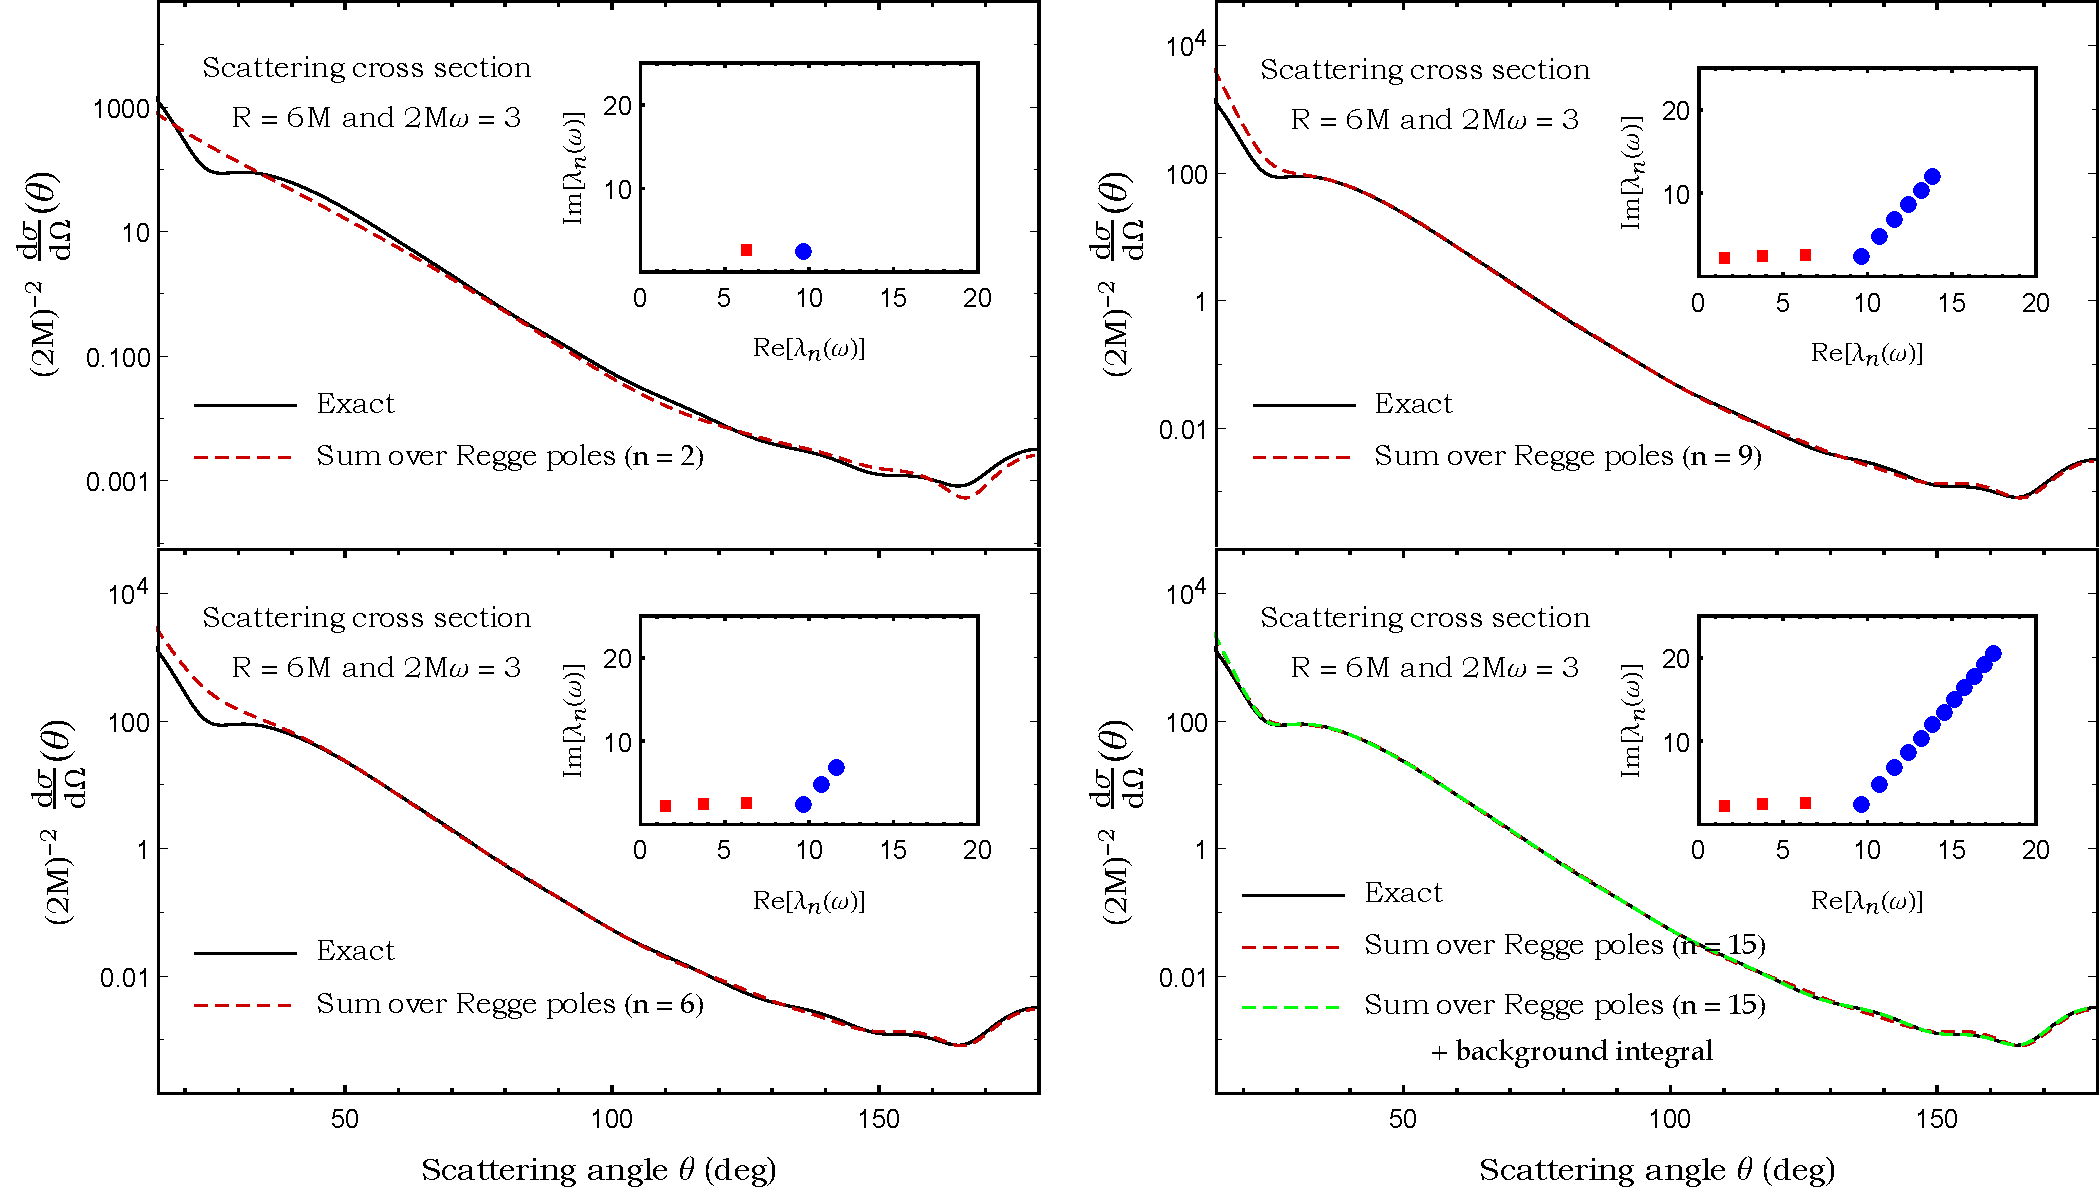
\includegraphics[scale=0.50]{Scattering_Cross_Section_R_6_2Mw_3}
\caption{\label{S_0_R_6_2Mw_3_Exact_vs_CAM} The scalar cross section of a compact bodies for $2M\omega=3$ and $R=6M$, its Regge pole approximation and the background integral contribution. The plots show the effect of including successively more Regge poles (plots 1--3). In the final plot, the background integral is added, giving a cross section which agrees well with the (regularized) partial-wave sum.}
\end{figure*}

Figure \ref{S_0_R_6_2Mw_16_Exact_vs_CAM} shows the neutron star model ($R/M = 6$) at the higher frequency of $M \omega = 8$. The first plot shows that, in this case, including just two Regge poles is yields a poor approximation. With 20 Regge poles, the primary peak of the rainbow, the first supernumerary, and the shadow region are well captured, but at smaller angles ($\theta  \lesssim 40^\circ$) there is no agreement. With 42 Regge poles, but no background integral, the agreement is excellent for $\theta \gtrsim 30^\circ$. Finally, with 81 Regge poles and the background integral included, the CAM result is again indistinguishable from the partial-wave result on the plot.

\begin{figure*}%[h!]
 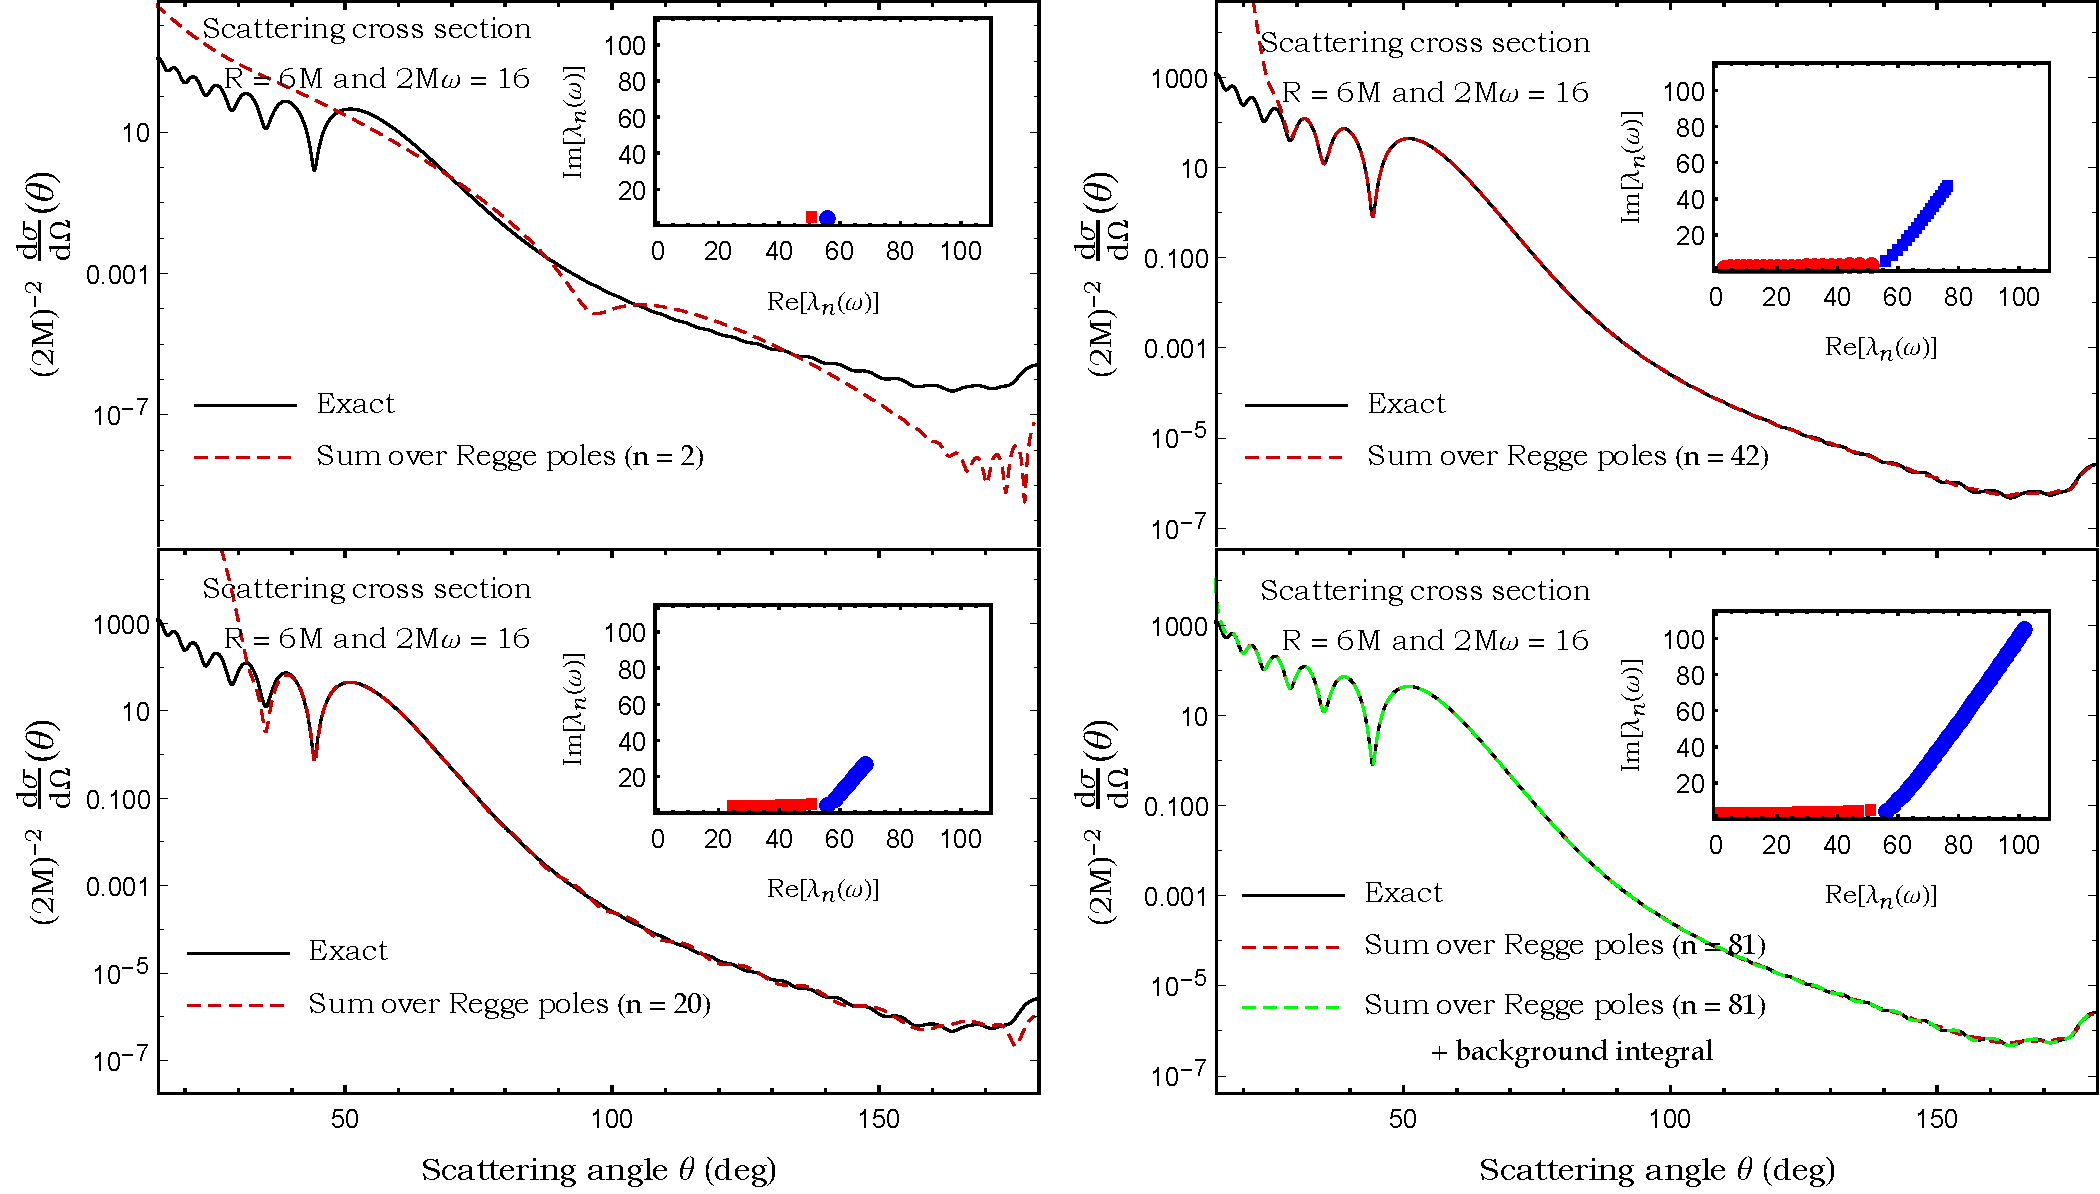
\includegraphics[scale=0.50]{Scattering_Cross_Section_R_6_2Mw_16}
\caption{\label{S_0_R_6_2Mw_16_Exact_vs_CAM} The scalar cross section of a compact bodies for $2M\omega=16$ and $R=6M$, its Regge pole approximation and the background integral contribution.}
\end{figure*}

Figure \ref{S_0_R_6_2Mw_16_Exact_vs_CAM} shows the cross section for an Ultra Compact Object with $R/M = 2.26$ at the `low' frequency of $M \omega = 3/2$. In this case, the rainbow angle exceeds $180^\circ$, and there is both a light-ring and a trapping region (see Fig.~\ref{fig:Veff}). The cross section exhibits regular orbiting oscillations with angle $\theta$. The angular width is consistent with generation by the light-ring (i.e.~ the peak in the potential barrier). The second plot shows that including just 3 modes from each of the three branches leads to a good description of scattering at large angles $\theta \gtrsim 100^\circ$. As there is no shadow region in this case, the cross section at large angles in non-negligible. For $R/M = 2.26$, the cross section at the antipodal point ($\theta = 180^\circ$) is a factor of $> 10^6$ larger than in the $R/M = 6$ case. The final plot shows that excellent agreement with the partial-wave results is obtained, for $\theta \gtrsim 20^\circ$, by summing over $27$ poles.

\begin{figure*}%[h!]
\centering
 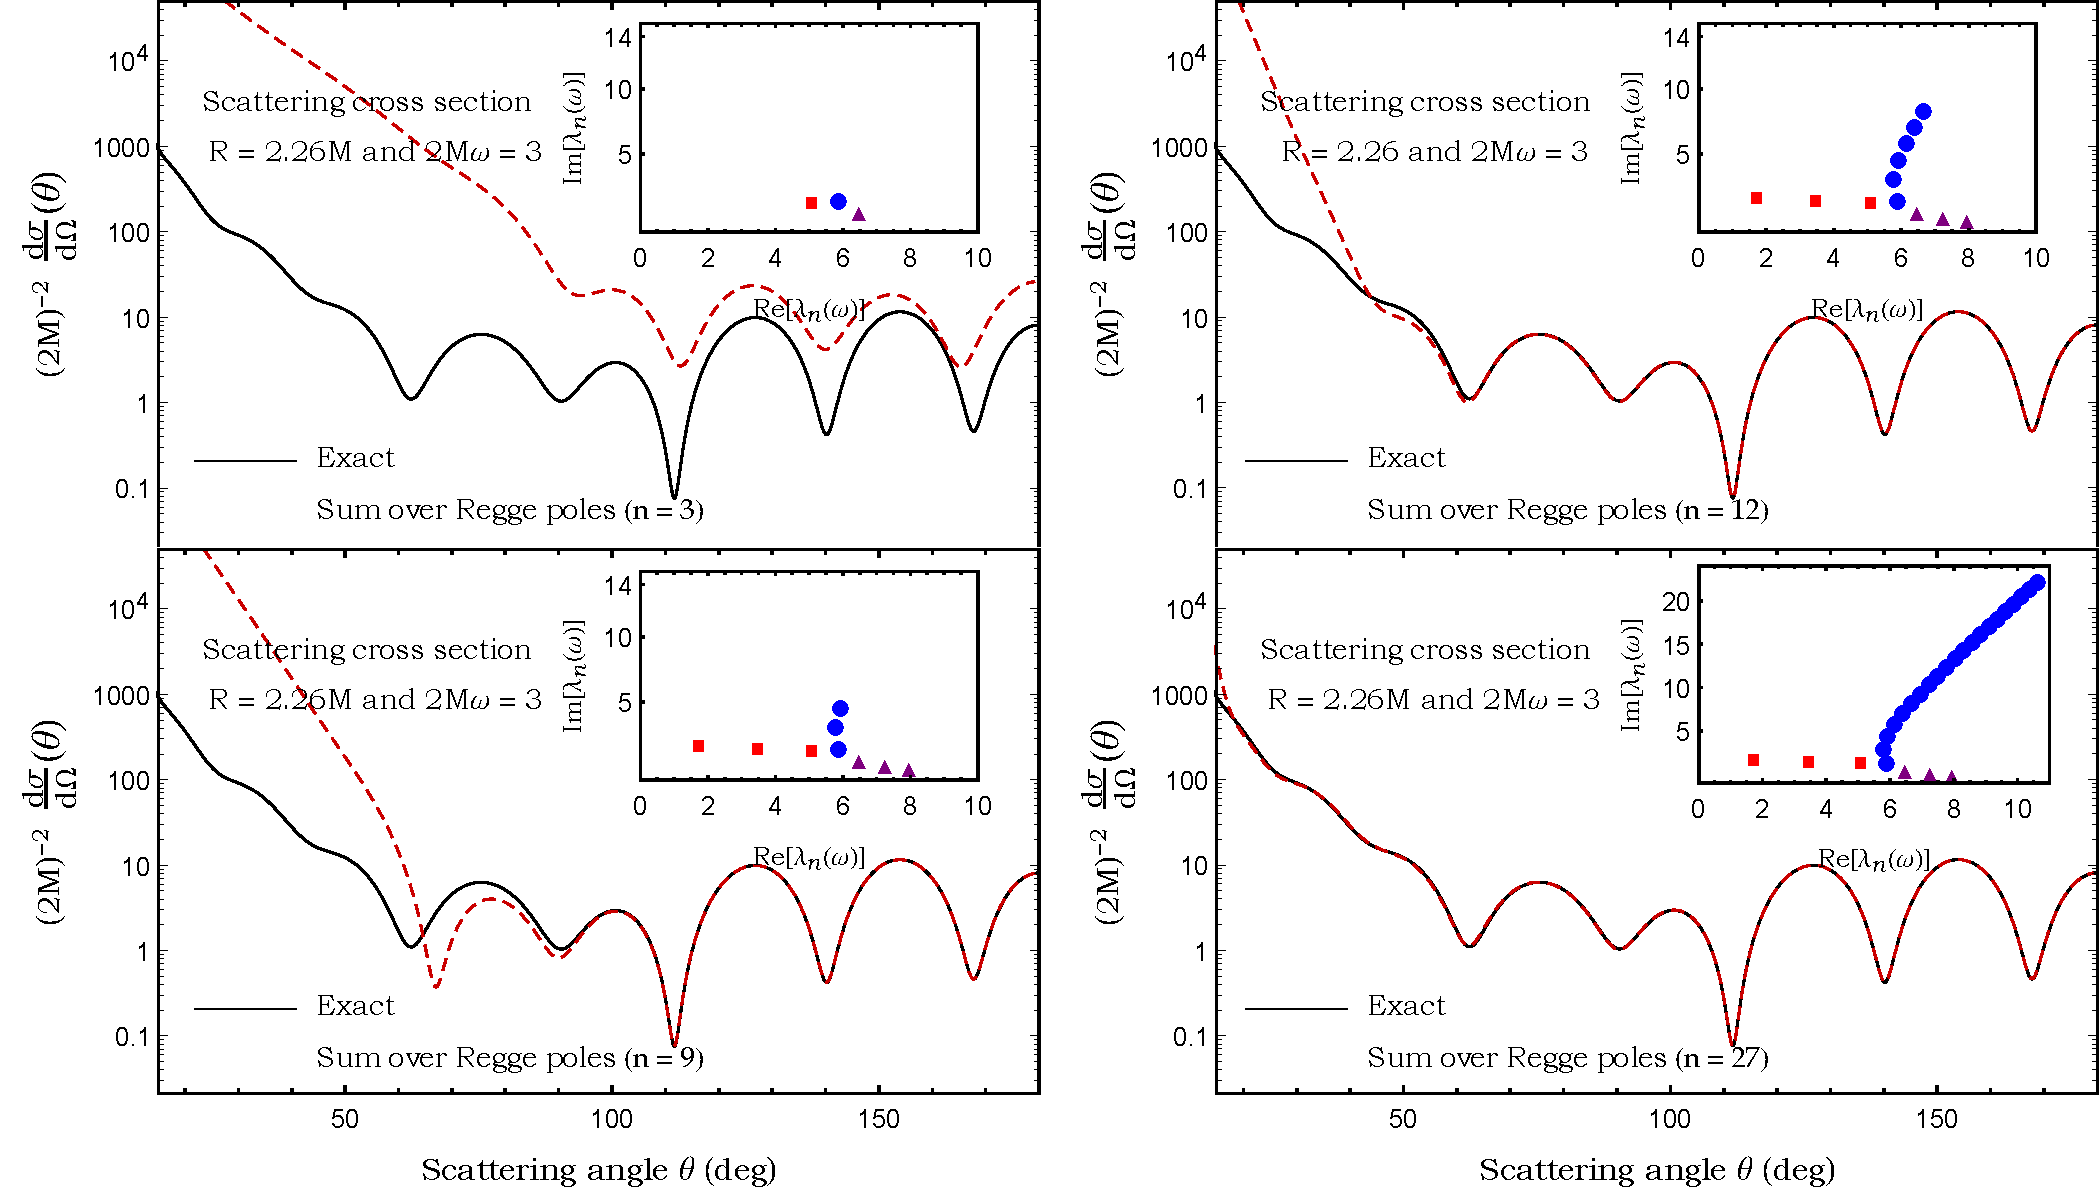
\includegraphics[scale=0.50]{Scattering_Cross_Section_R_2-dot-26_2Mw_3}
\caption{\label{S_0_R_2-dot-26_2Mw_3_Exact_vs_CAM} The scalar cross section of a very compact bodies for $2M\omega=3$ and $R=2.26M$ and its Regge pole approximation.}
\end{figure*}

Figure \ref{S_0_R_2-dot-26_2Mw_6_Exact_vs_CAM} shows the cross section for an UCO at the higher frequency of $M \omega = 8$. In this case, the cross section is non-negligible at all angles, and there is evidence for interference between oscillations of comparable amplitudes and widths. Summing 31 Regge poles leads to good agreement for the cross section for angles $\theta \gtrsim 35^\circ$. As before, it is necessary to include the background integral as well to obtain agreement at smaller angles.

\begin{figure*}%[h!]
\centering
 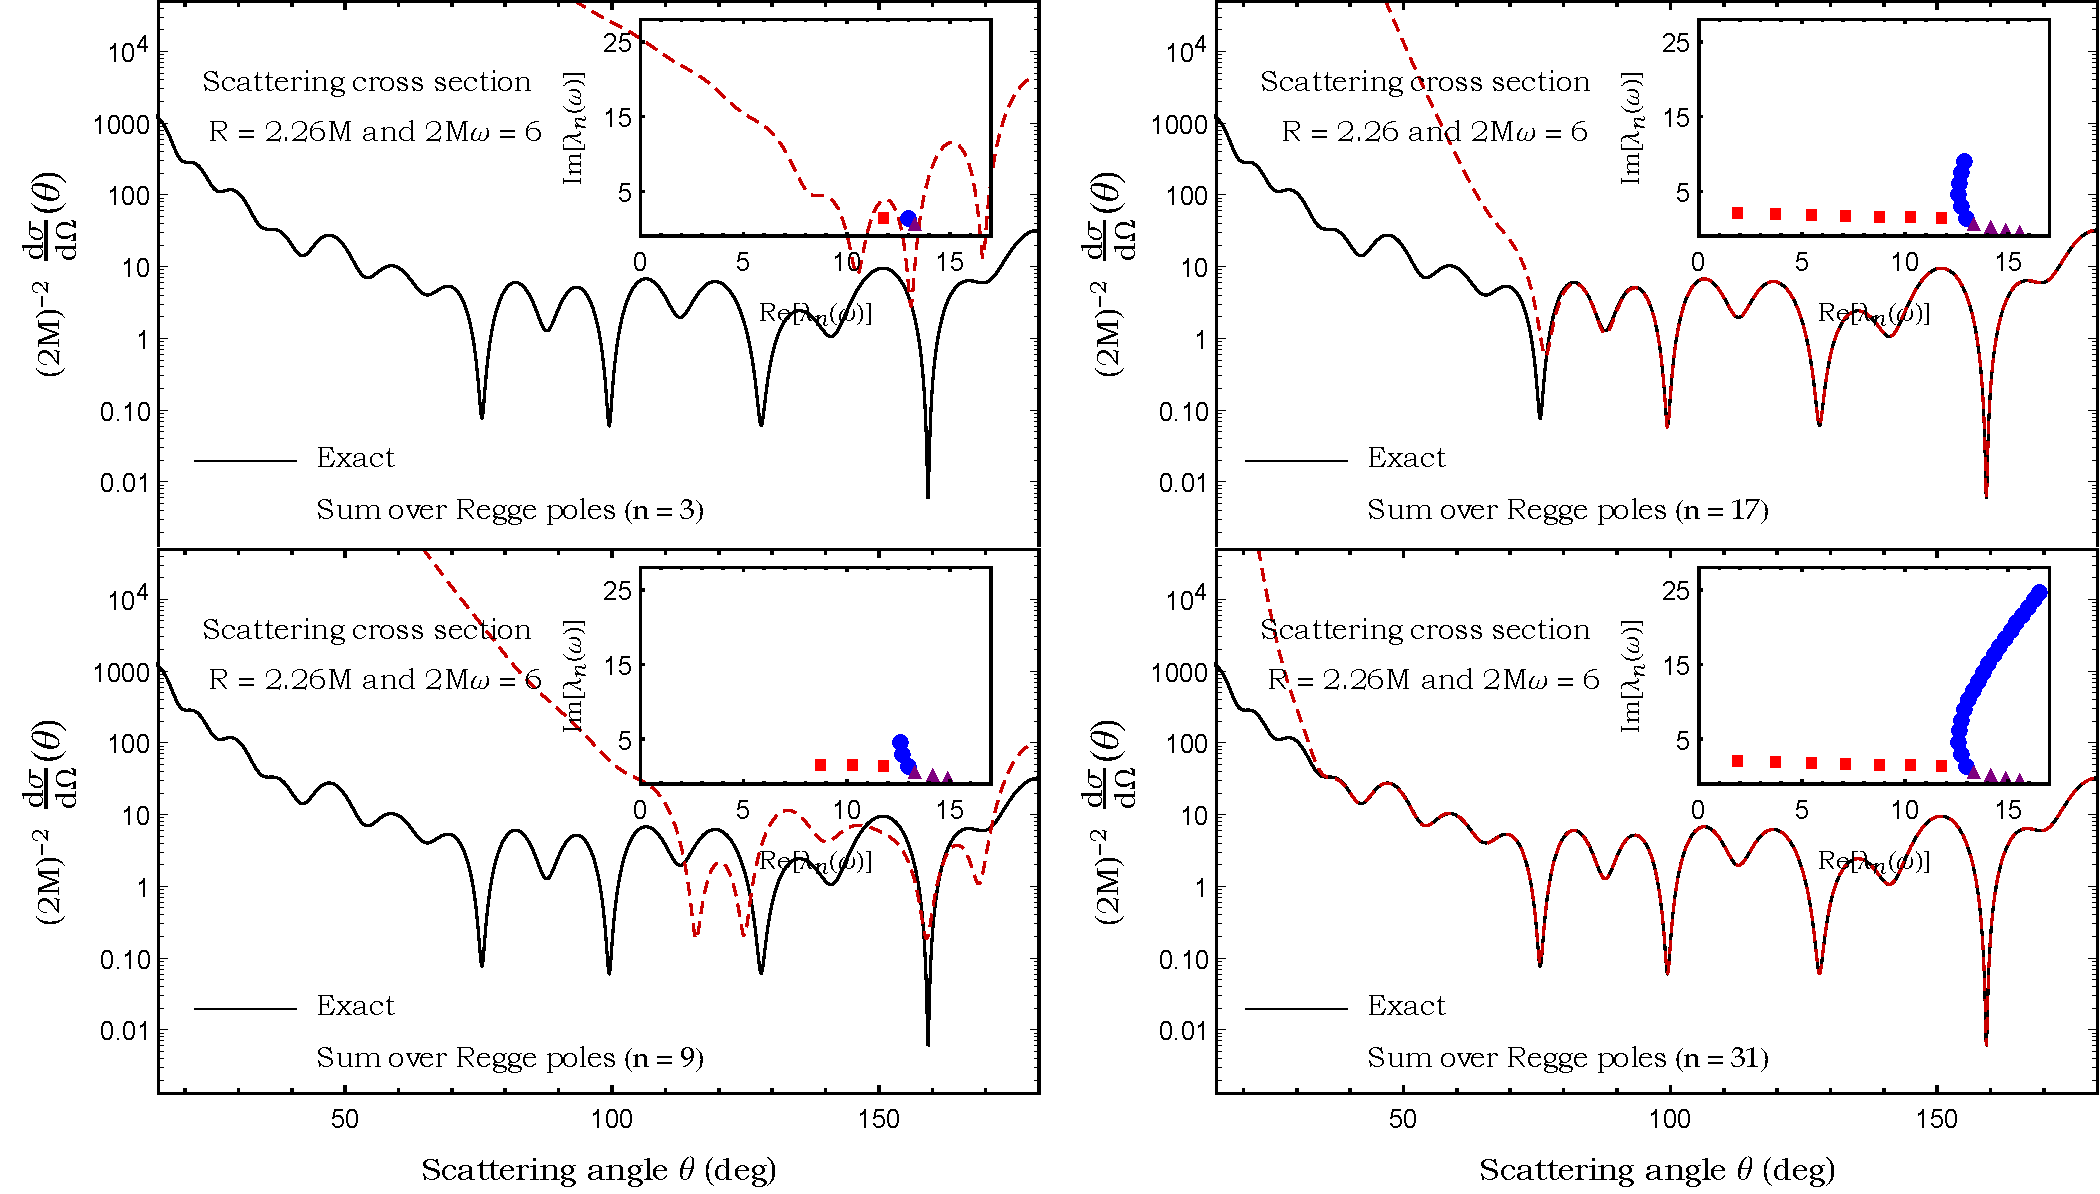
\includegraphics[scale=0.50]{Scattering_Cross_Section_R_2-dot-26_2Mw_6}
\caption{\label{S_0_R_2-dot-26_2Mw_6_Exact_vs_CAM} The scalar cross section of a very compact bodies for $2M\omega=6$ and $R=2.26M$ and its Regge pole approximation.}
\end{figure*}

Figures \ref{Rainbow_Cross_Section_R_6_2Mw_16} and \ref{Diff_Contribution_Cross_Section_R_2-dot-26_2Mw_6} show the relative magnitudes of the contributions from the different branches of Regge poles. For $R/M = 6$ (Fig.~ \ref{Rainbow_Cross_Section_R_6_2Mw_16}) the surface-wave and broad-resonance amplitudes are similar in magnitude, and similar in magnitude to their sum. There is a difference in phase between these amplitudes which generates the peaks and troughs of the rainbow-scattering pattern.


\begin{figure}%[h!]
\centering
 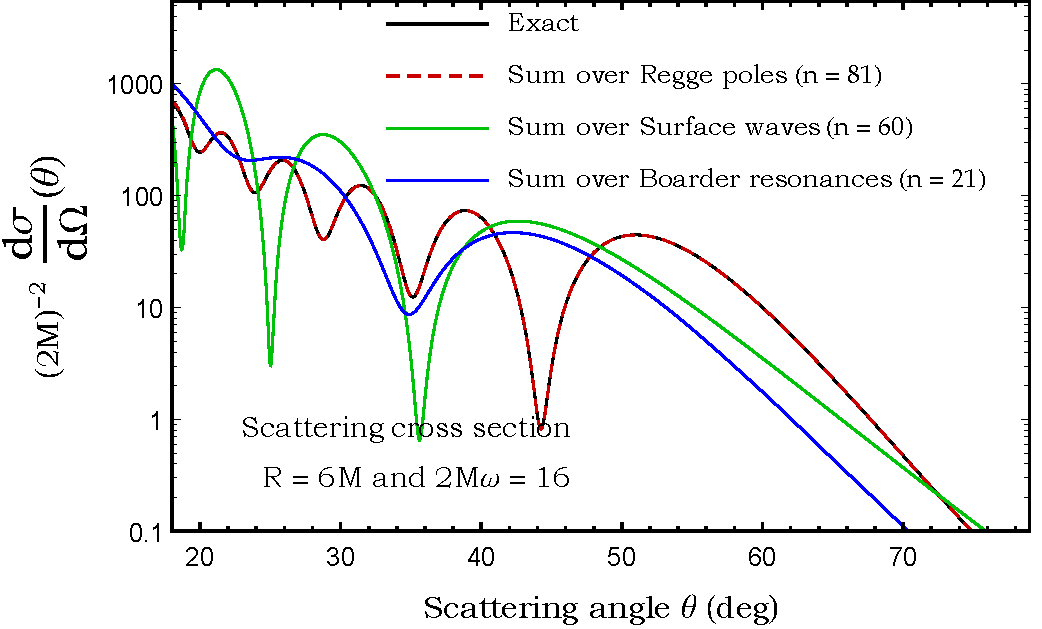
\includegraphics[scale=0.50]{Rainbow_Cross_Section_R_6_2Mw_16}
\caption{\label{Rainbow_Cross_Section_R_6_2Mw_16} Rainbow scattering for compact bodies for $2M\omega=16$ and $R=6M$, its Regge pole approximation and different contributions of the sum over Regge poles.}
\end{figure}

For $R/M = 2.26$ (Fig.~\ref{Diff_Contribution_Cross_Section_R_2-dot-26_2Mw_6}), however, the amplitudes  from the three branches are comparable in magnitude, but their sum is several orders-of-magnitude smaller. In other words, there is some delicate cancellation occurring between the contributions from the branches, suggesting that the CAM approach used here is not an efficient method for computing the cross section in this case.

\begin{figure}%[h!]
\centering
 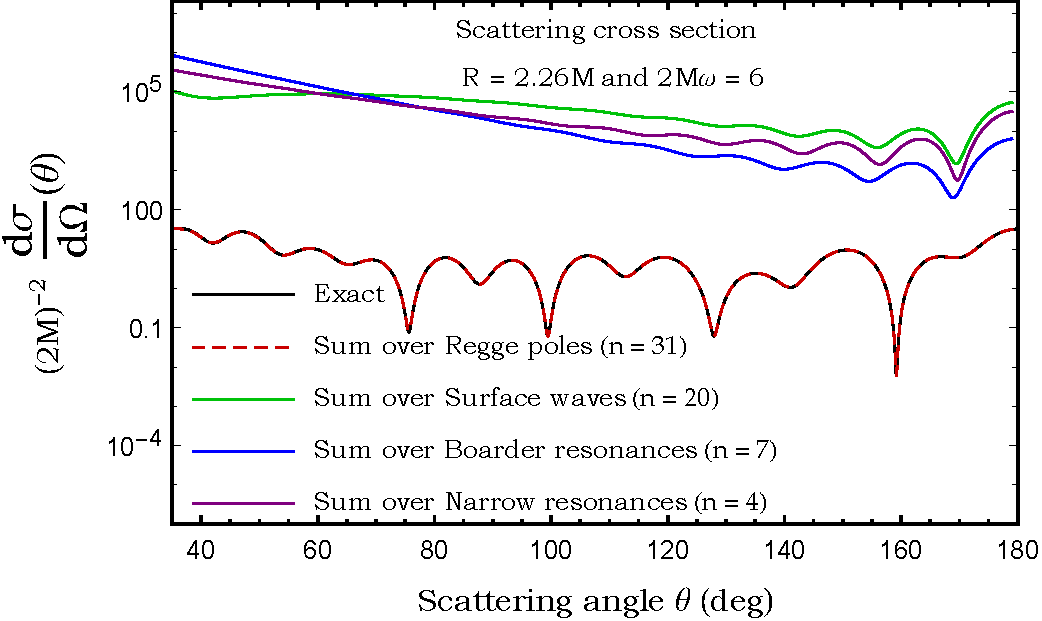
\includegraphics[scale=0.50]{Diff_Contribution_Cross_Section_R_2-dot-26_2Mw_6}
\caption{\label{Diff_Contribution_Cross_Section_R_2-dot-26_2Mw_6} Rainbow scattering for compact bodies for $2M\omega=16$ and $R=2.26M$, its Regge pole approximation and different contributions of the sum over Regge poles.}
\end{figure}


\section{Discussion and conclusions\label{sec:conclusions}}

We have calculated the full spectrum of Regge poles for a compact body spacetime for the first time.

We find 2 distinct branches - - in the case $R > 3M$, and a third branch of narrow resonances appears for UCO.

Confident that there are no additional poles in the first quadrant with imaginary parts less than (blah), for two reasons. First, we have scanned across the domain using the scanning method. Second, we obtain an excellent agreement, which would not be the case if poles in this domain had been missed.

Links between QNMs and Regge poles. Further examination.

Through a WKB method, we have obtained qualitative understanding of the broad resonances, finding that the imaginary part is predicted, with a certain degree of accuracy, from the discontinuity in the potential at the surface of the body. Further work is need on modelling the surface-wave branch, the narrow resonances. Taking the WKB method to higher orders will presumably improve the accuracy.


Complementary method. Not efficient method at present. Convergence of the sum is not as rapid as in the BH case, due to the branch of broad resonances close to the real axis. Neither have we obtained an approximation has powerful as that of Ould Elhadj and Folacci for describing the orbiting phenomenon. In the case of Mie scattering, a powerful resummation approach is that of Regge-Debye poles, reducing to one branch of poles of higher order. This is a possible direction for future work.

We have examined the case of $R=2.26M$, which is above the Buchdahl bound but nevertheless below ... blah blah, work in Tom's text.





\acknowledgments
M. O. E. H. wish to thank Antoine Folacci for various discussions concerning this work. T.S.~acknowledges financial support from EPSRC. S.R.D.~acknowledges financial support from the European Union's Horizon 2020 research and innovation programme under the H2020-MSCA-RISE-2017 Grant No.~FunFiCO-777740, and from the Science and Technology Facilities Council (STFC) under Grant No.~ST/P000800/1.



\bibliography{rainbowCAM}
\bibliographystyle{apsrev4-1}

\end{document}
